\chapter{Interface graphique (bonus)}\label{chap:interface}

\section{Principes}
L'interface est une application web monopage (HTML, CSS, JavaScript sans framework) servie par la plateforme. Elle
consomme \emph{directement} les services : un petit client SOAP en JavaScript (\code{soap.js}) construit les enveloppes
avec l'en-tête WS-Security et convertit les réponses XML, tandis que les services REST sont appelés en JSON. Le
diagramme BPMN est affiché avec \textbf{bpmn-js}, embarqué dans l'application, ce qui permet de suivre une instance
en direct. La charte reprend le bleu de l'INPT. Après connexion, le menu s'adapte au rôle :

\begin{table}[htbp]
\centering\small
\caption{Écrans par acteur}
\begin{tabularx}{\textwidth}{@{}lY@{}}
\toprule
\textbf{Acteur} & \textbf{Écrans} \\
\midrule
Étudiant & Offres ouvertes à son année d'études, avec type de stage (badge et filtre), score d'adéquation et motifs d'incompatibilité ; dépôt de candidature (déclenche le
  processus) ; suivi des candidatures (chronologie en 5 étapes), complément et annulation ; notifications ; « Mon stage » (progression,
  comptes rendus, évaluations) ; « Mon profil » (coordonnées et compétences modifiables) \\
Entreprise & Candidatures à évaluer (profil, compétences, lettre, CV) et formulaire de décision ; publication (choix
  du type de stage) et clôture d'offres (SOAP) ; candidatures reçues ; stagiaires, démarrage du stage et évaluations ; « Mon profil » (coordonnées et contact modifiables) \\
Responsable & Tableau de bord ; processus BPMN et instances (diagramme surligné, trace, variables) ; incidents
  (relancer, abandonner) ; gestion des étudiants et entreprises (SOAP) ; offres (avec leur type de stage), candidatures et stages ; supervision
  (pannes simulées, campagne de rappels) ; « Ma clé d'API » \\
\bottomrule
\end{tabularx}
\end{table}

\section{Parcours de l'étudiant}
\begin{figure}[H]
\centering
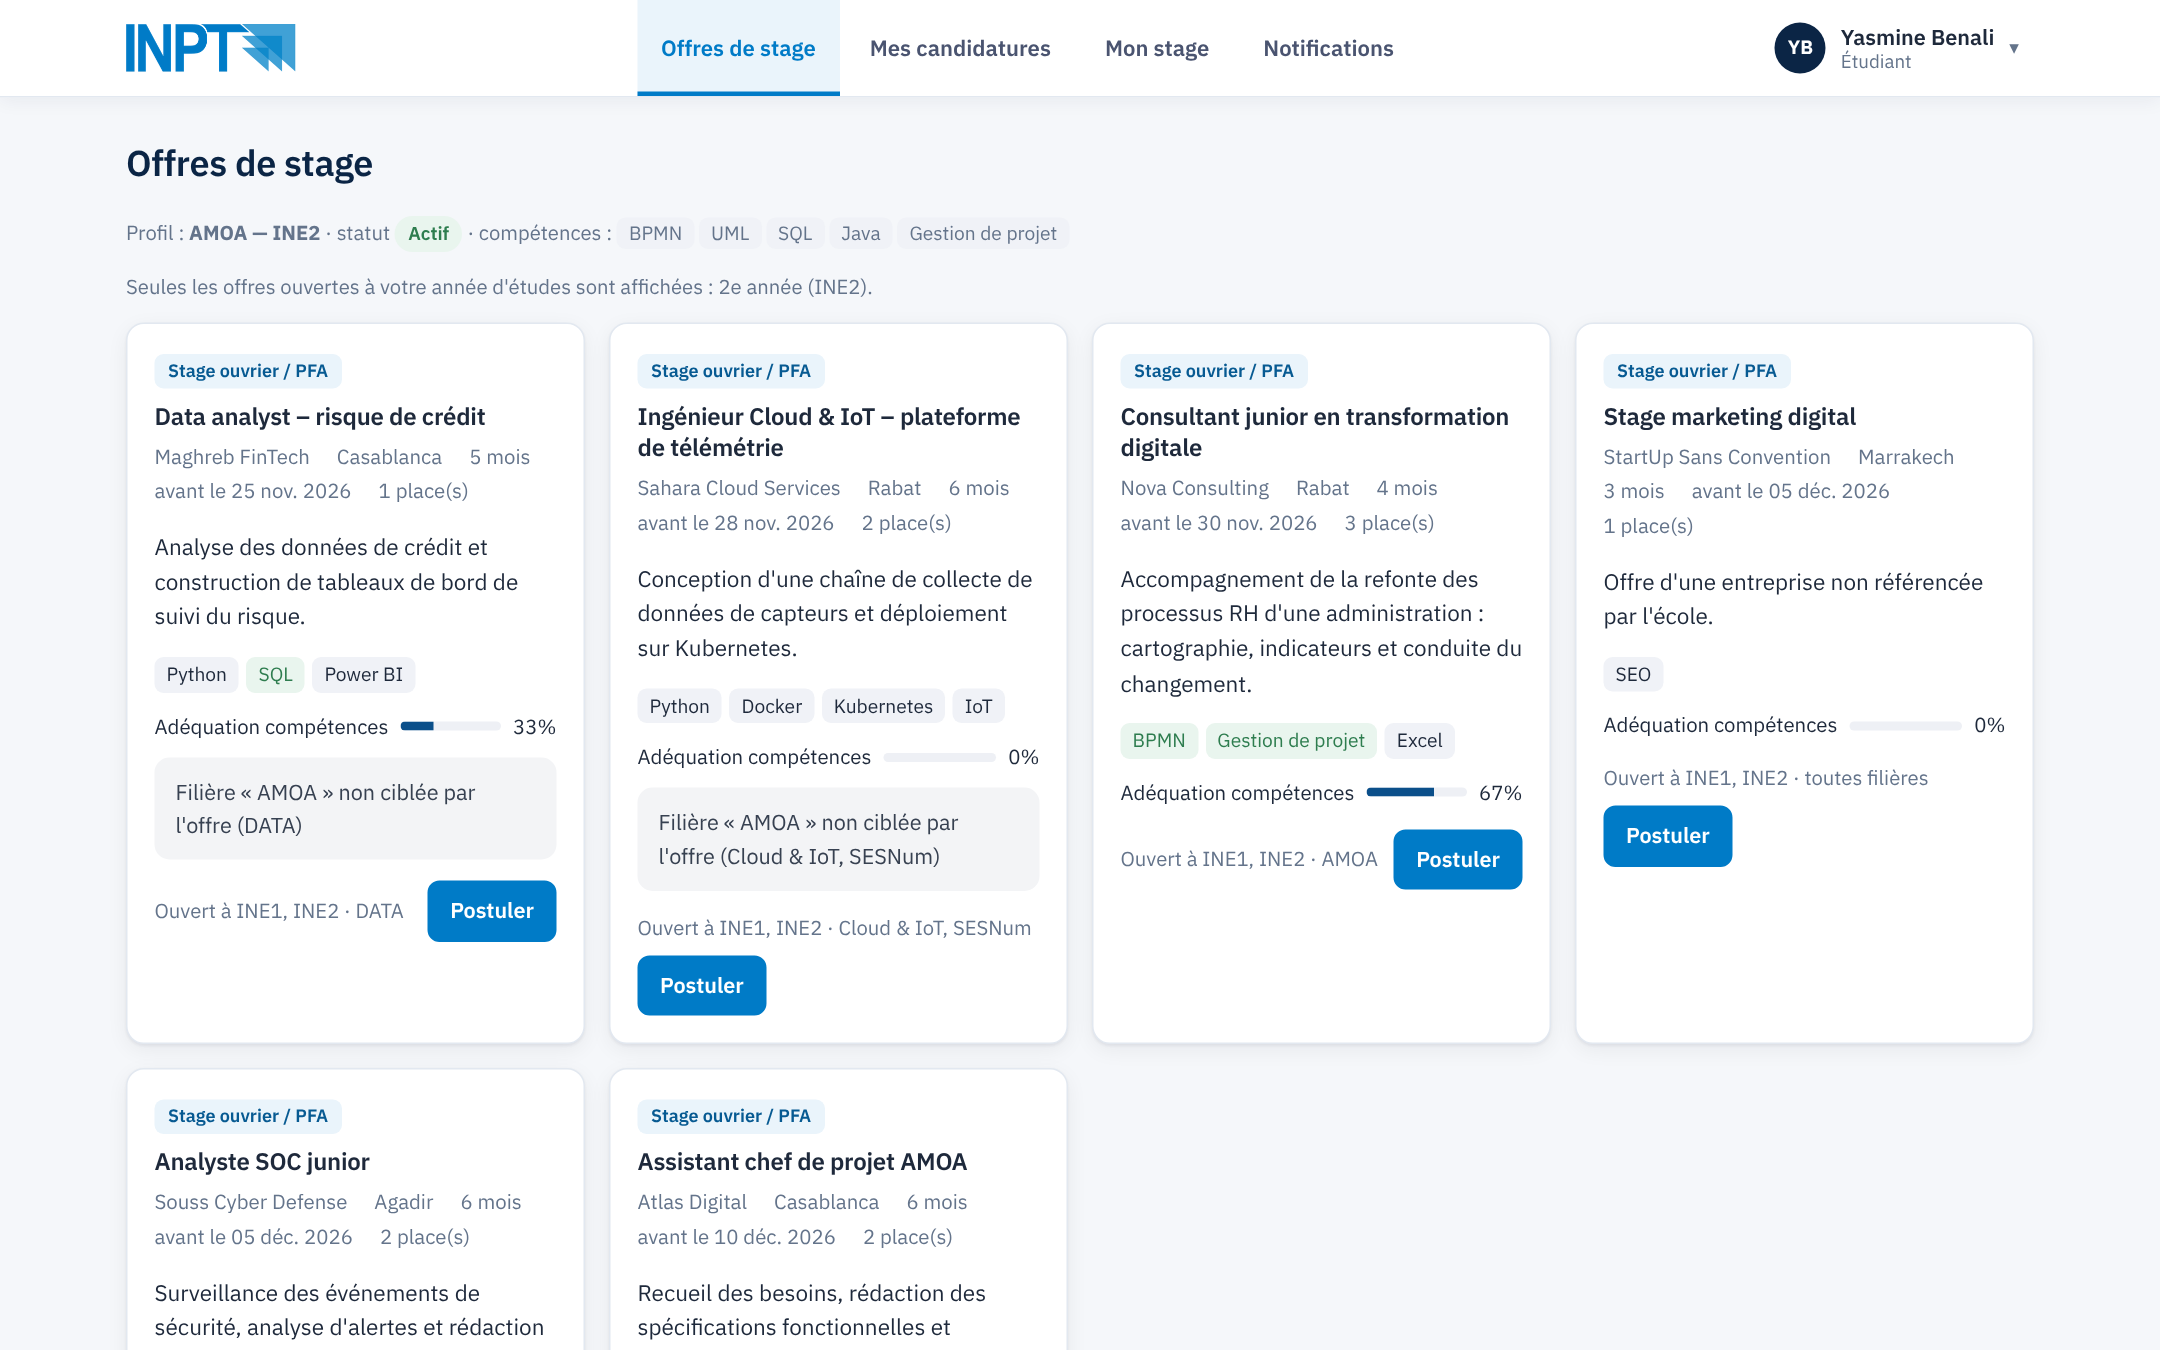
\includegraphics[width=0.92\textwidth]{figures/ui-etudiant-offres.png}
\caption{Offres de stage : score d'adéquation et motifs d'incompatibilité calculés par \code{verifierCompatibilite}}
\end{figure}

\begin{figure}[H]
\centering
\begin{minipage}{0.49\textwidth}\centering
  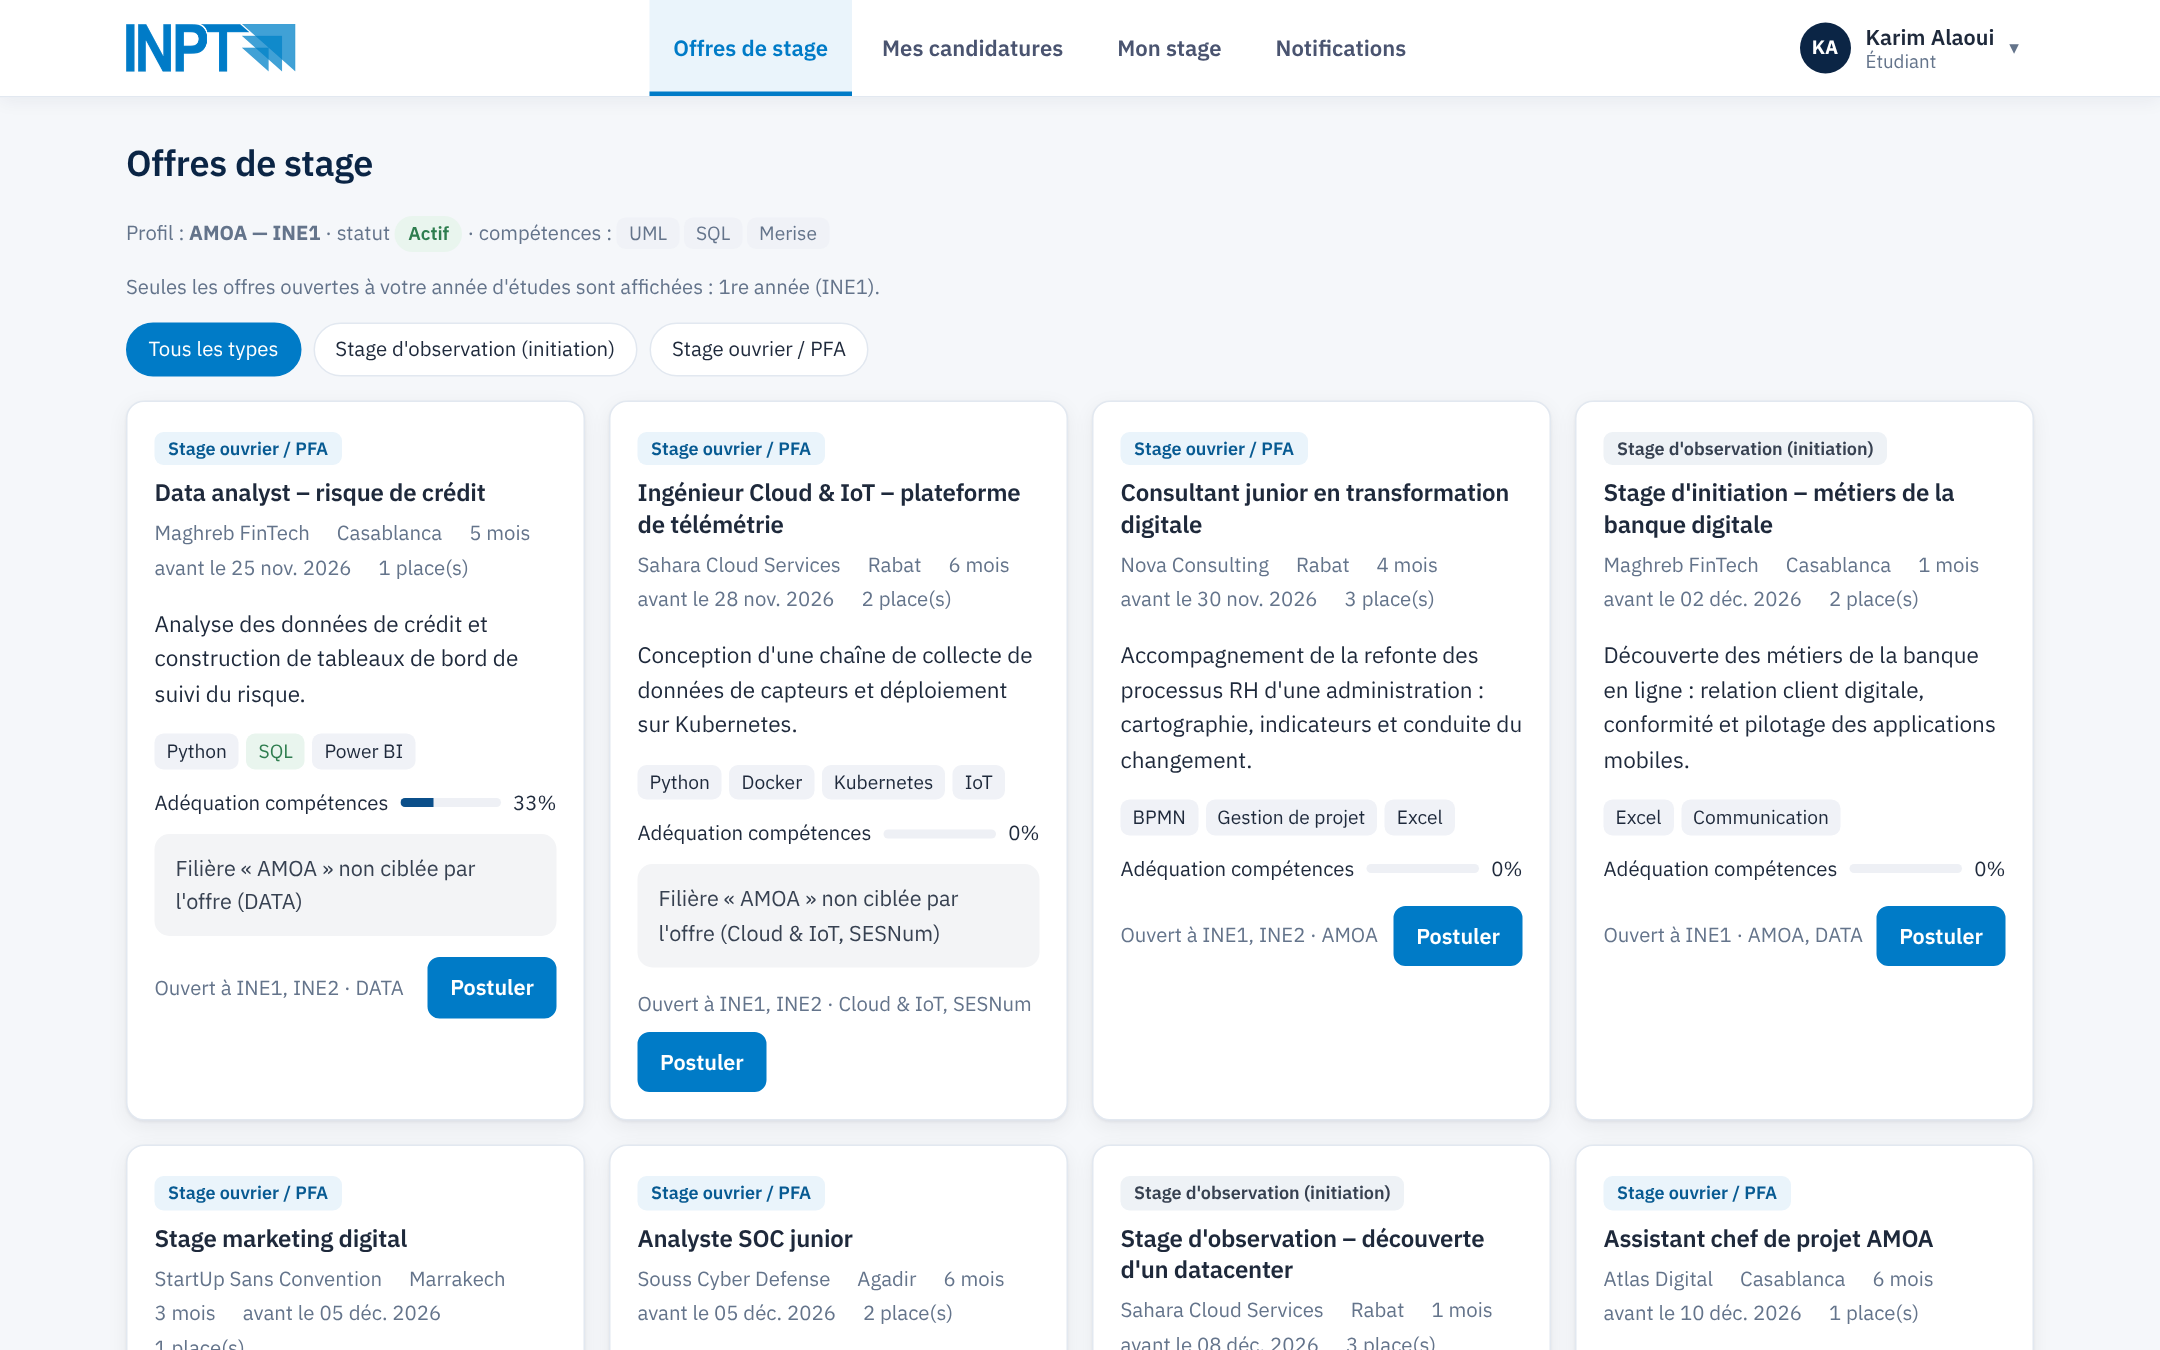
\includegraphics[width=\linewidth]{figures/ui-etudiant-offres-types.png}\\[-2pt]{\small (a) étudiant de 1re année : observation et ouvrier / PFA, filtre par type}
\end{minipage}\hfill
\begin{minipage}{0.49\textwidth}\centering
  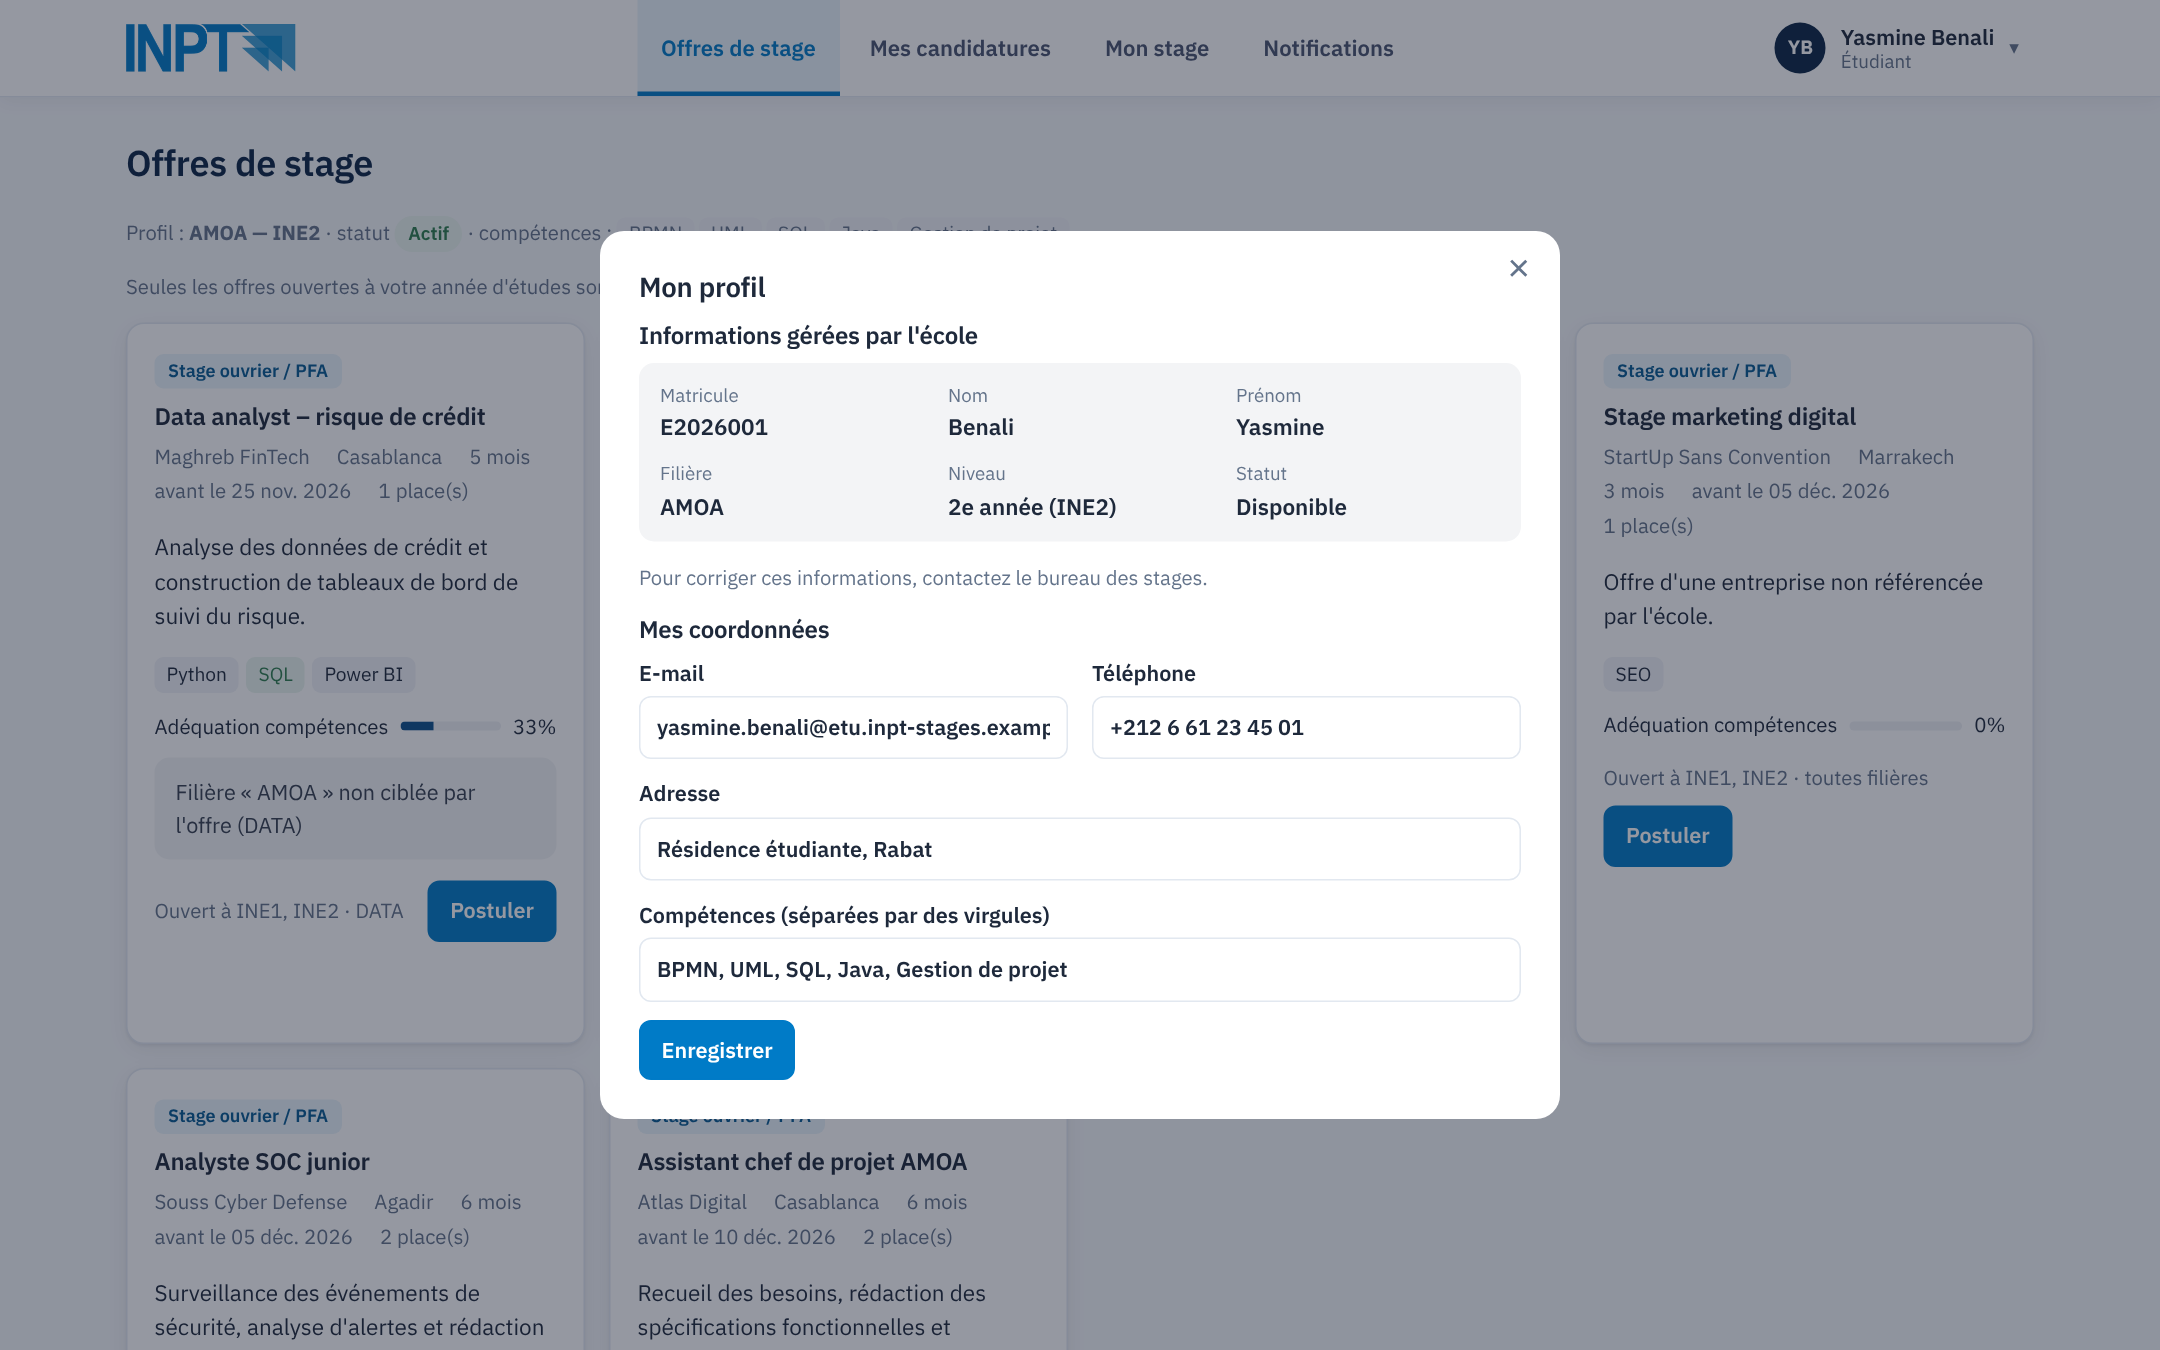
\includegraphics[width=\linewidth]{figures/ui-etudiant-profil.png}\\[-2pt]{\small (b) « Mon profil » : champs gérés par l'école en lecture seule}
\end{minipage}
\caption{Offres filtrées selon l'année d'études et profil de l'étudiant}
\end{figure}

\begin{figure}[H]
\centering
\begin{minipage}{0.49\textwidth}\centering
  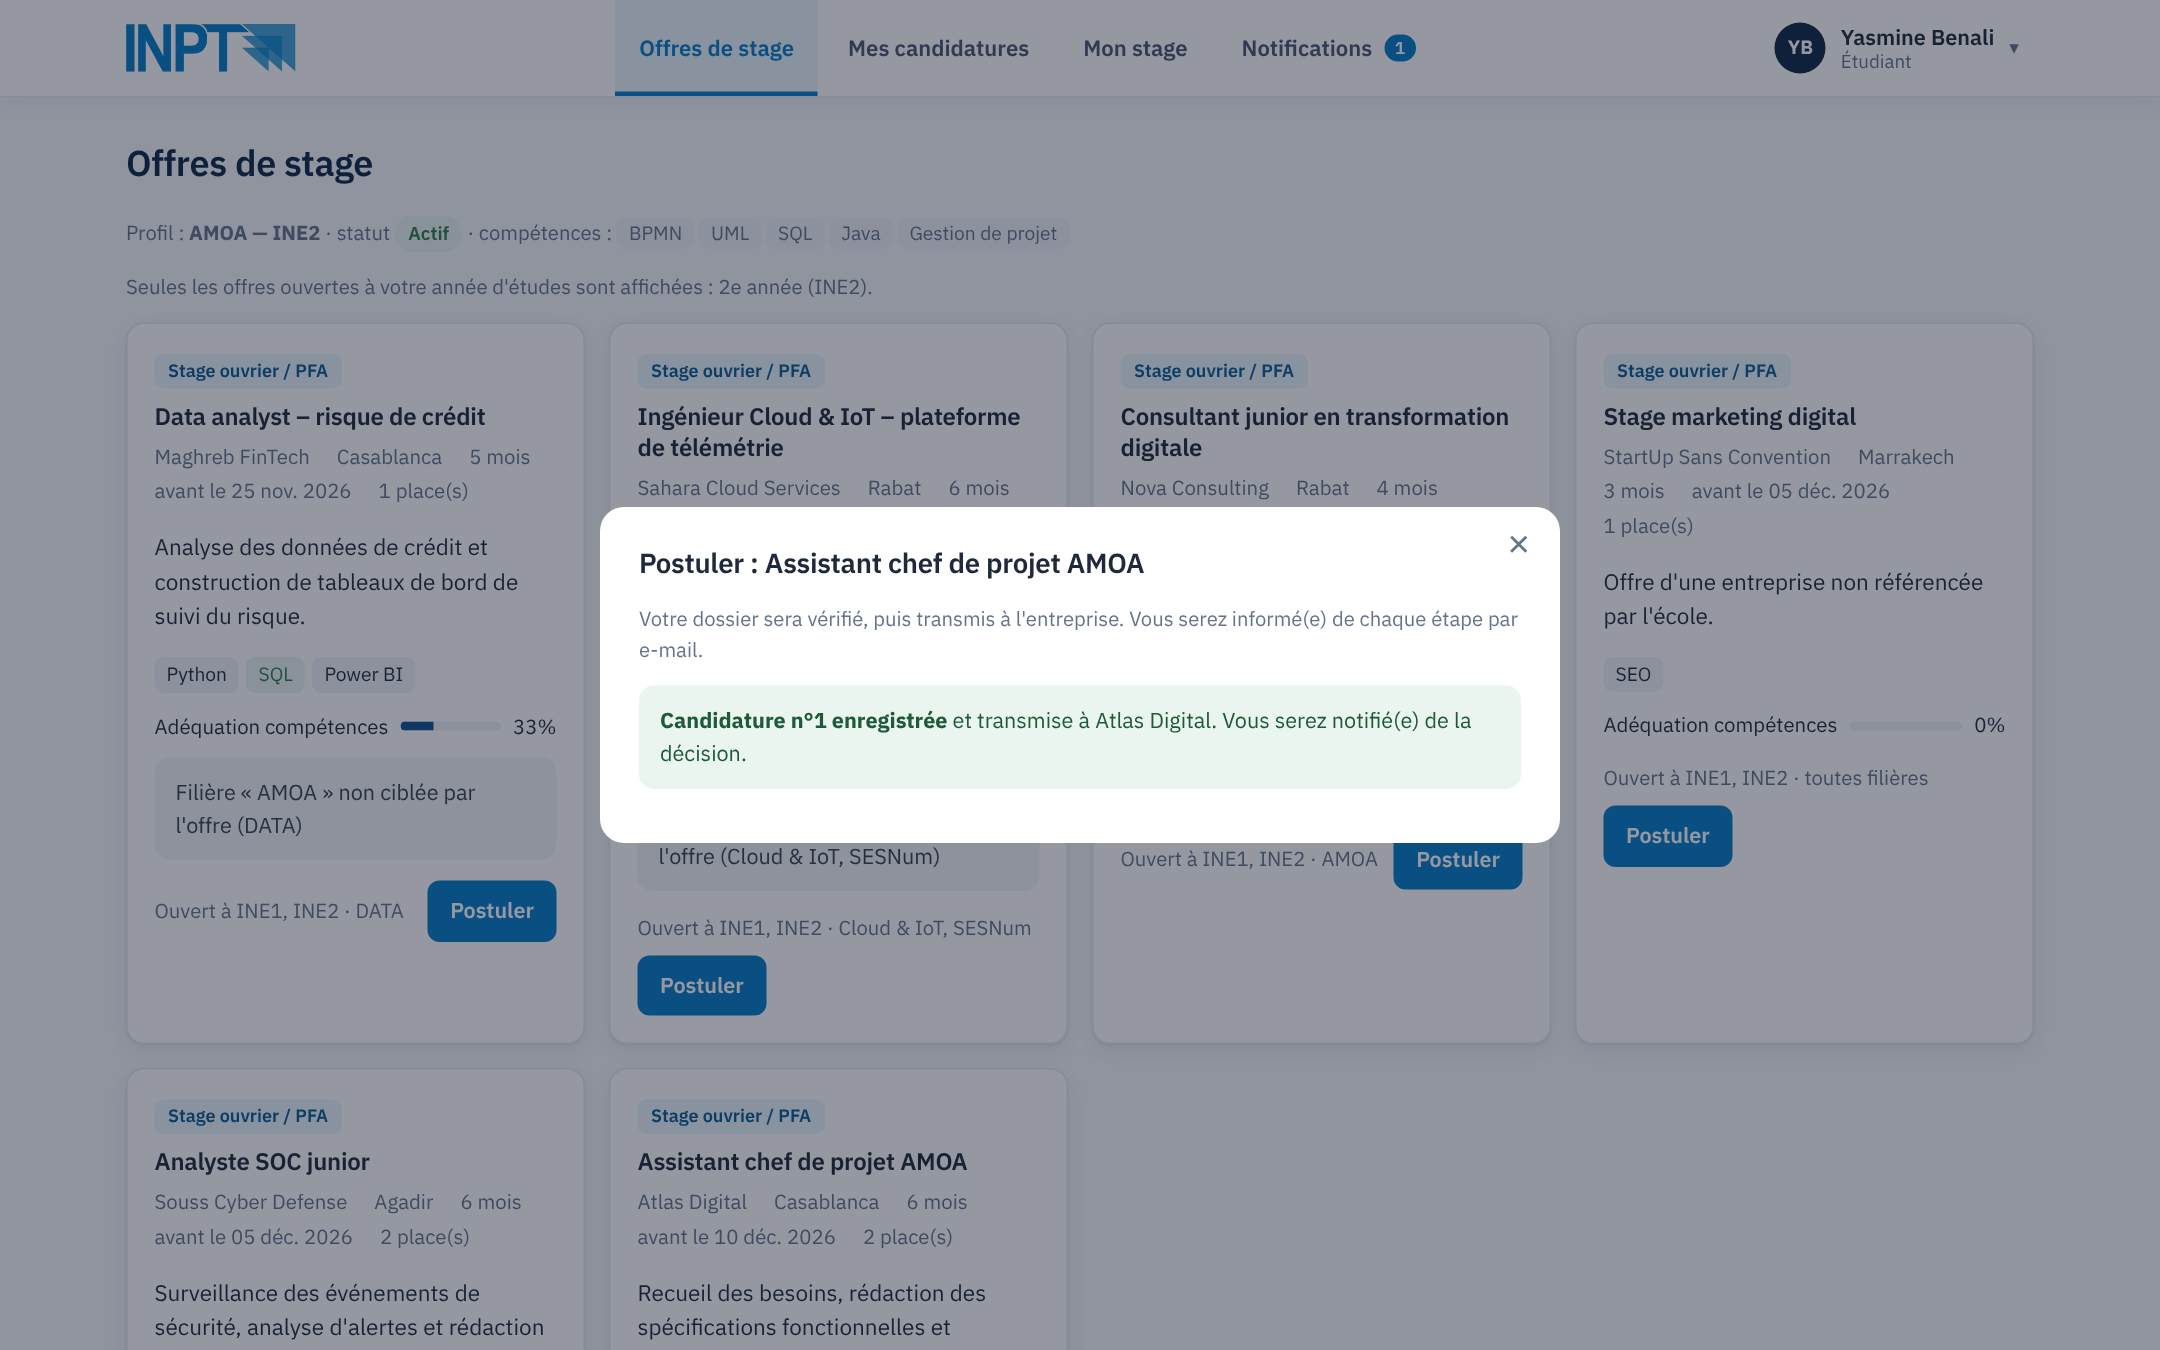
\includegraphics[width=\linewidth]{figures/ui-etudiant-postuler.png}\\[-2pt]{\small (a) candidature enregistrée}
\end{minipage}\hfill
\begin{minipage}{0.49\textwidth}\centering
  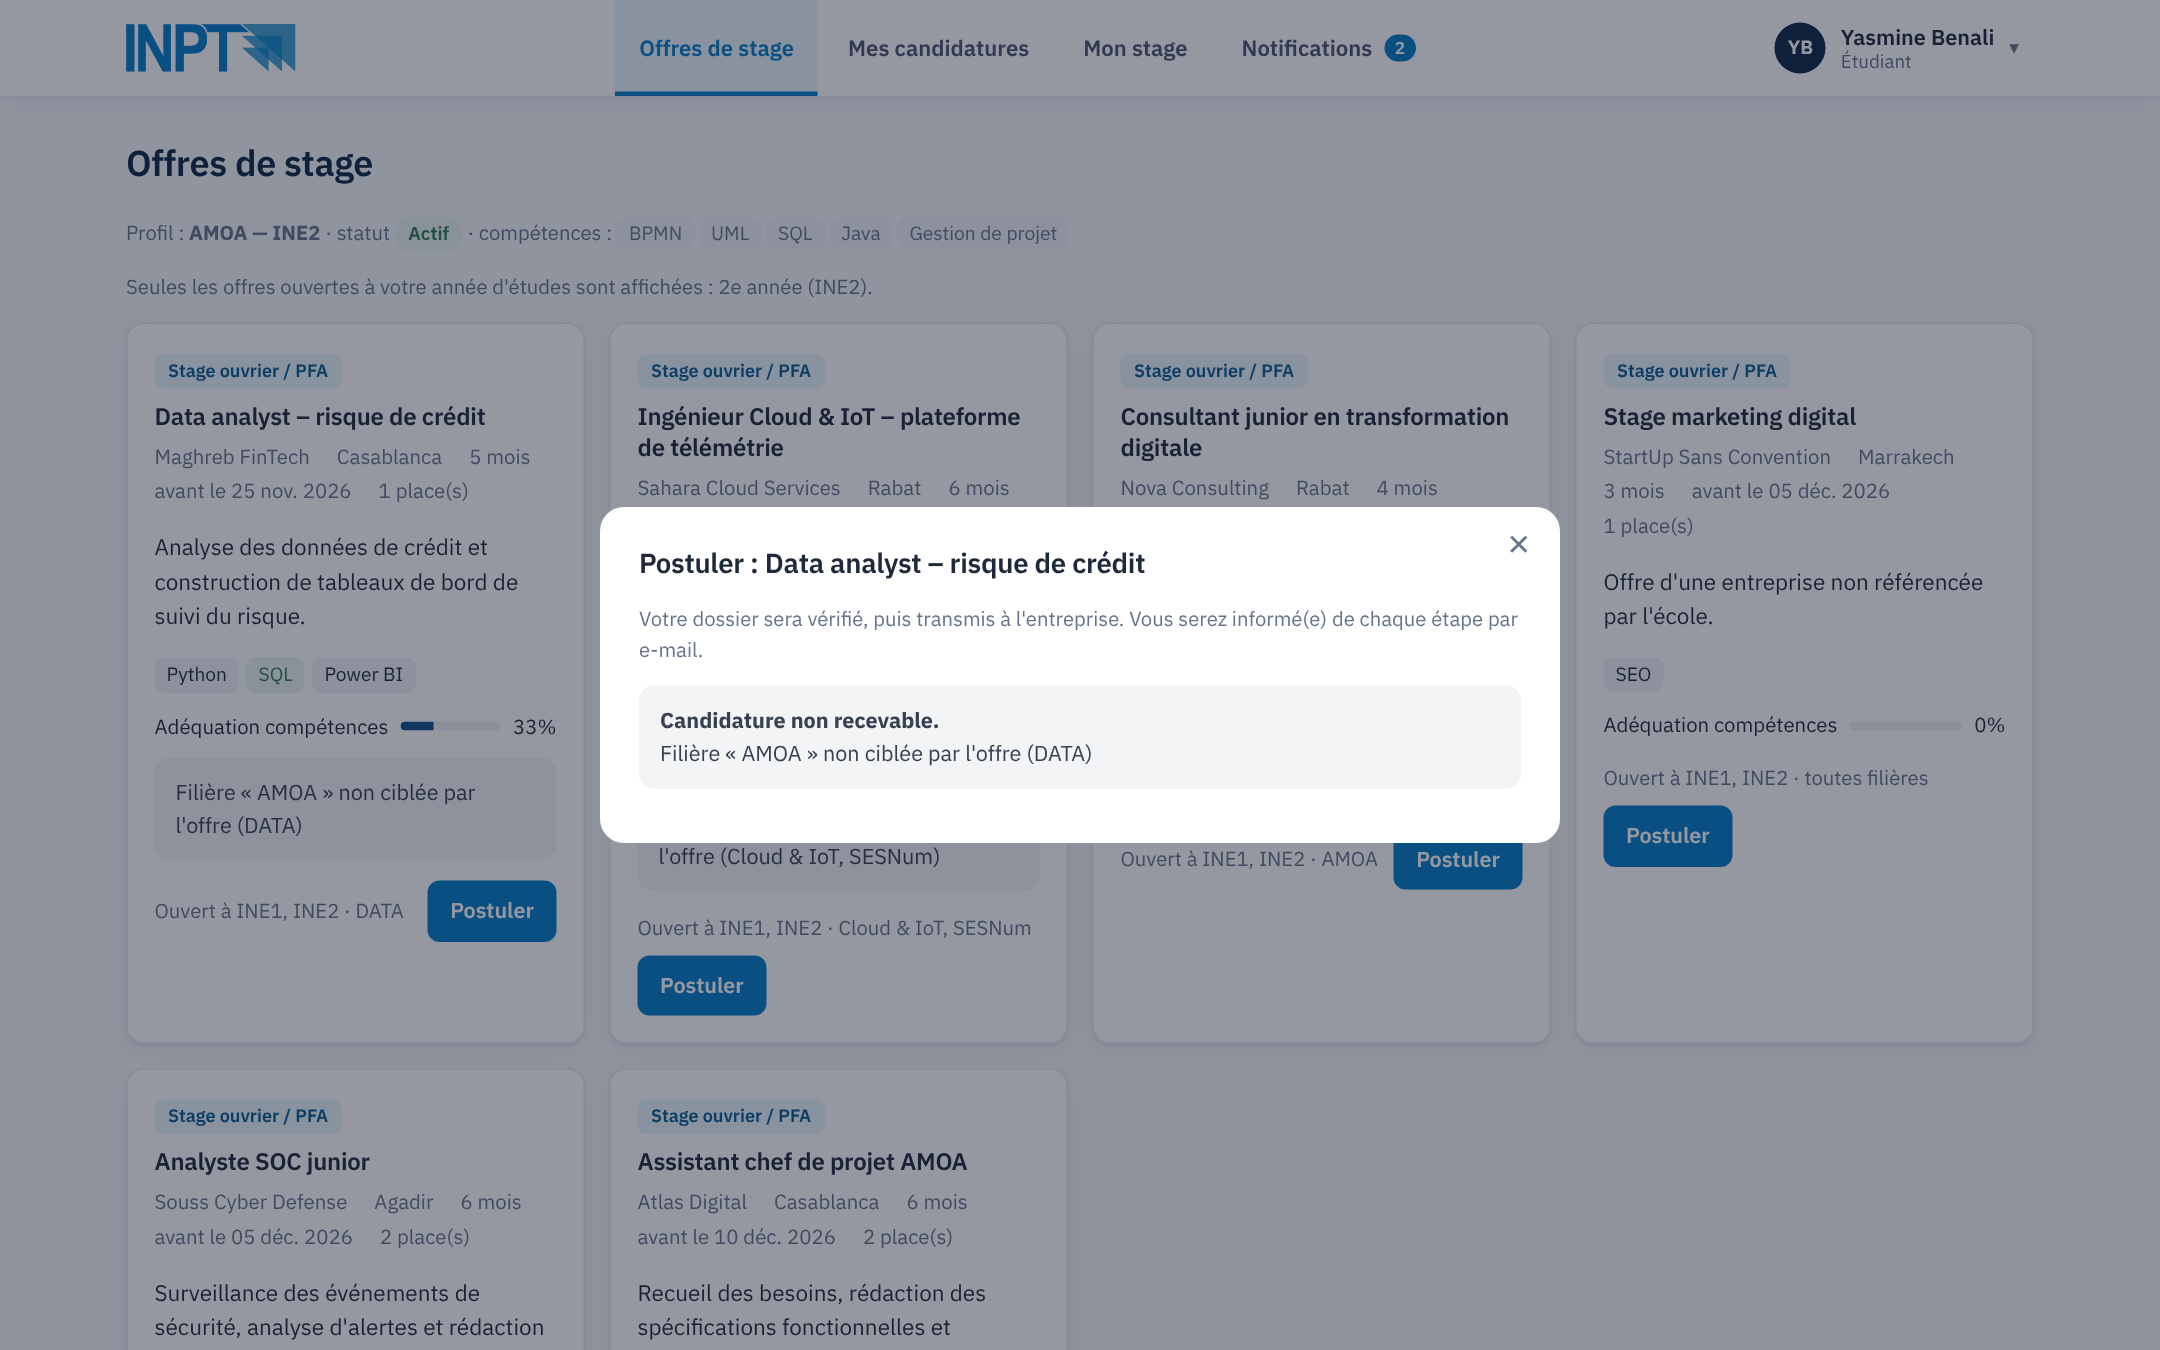
\includegraphics[width=\linewidth]{figures/ui-etudiant-rejet.png}\\[-2pt]{\small (b) rejet motivé par le processus}
\end{minipage}
\caption{Résultat d'une soumission de candidature}
\end{figure}

\begin{figure}[H]
\centering
\begin{minipage}{0.49\textwidth}\centering
  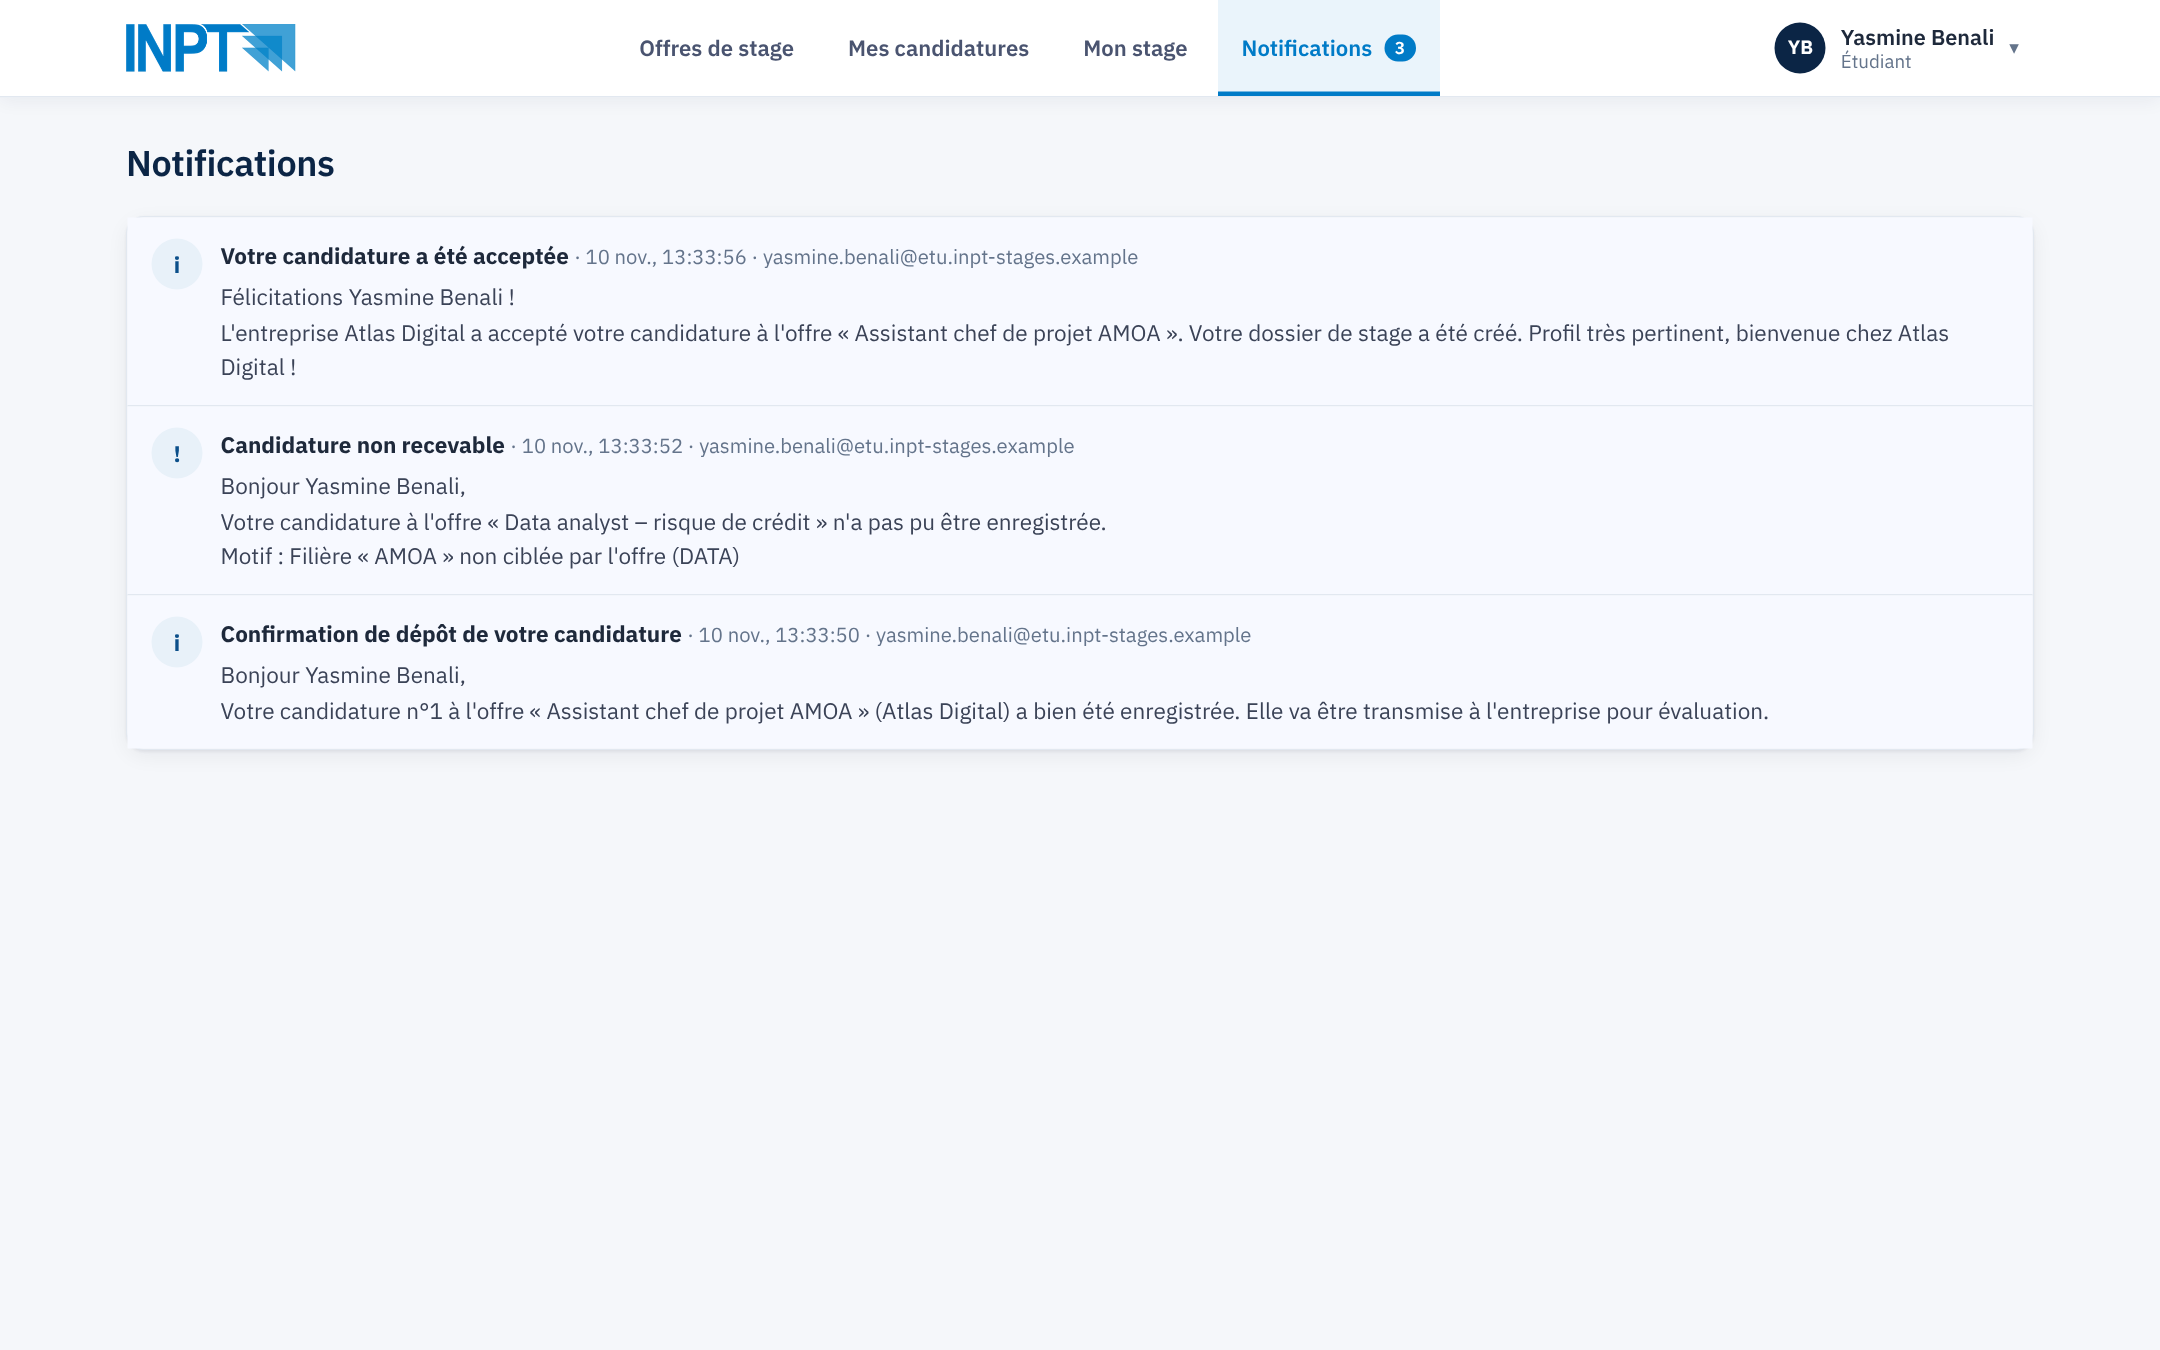
\includegraphics[width=\linewidth]{figures/ui-etudiant-notifications.png}\\[-2pt]{\small (a) notifications reçues}
\end{minipage}\hfill
\begin{minipage}{0.49\textwidth}\centering
  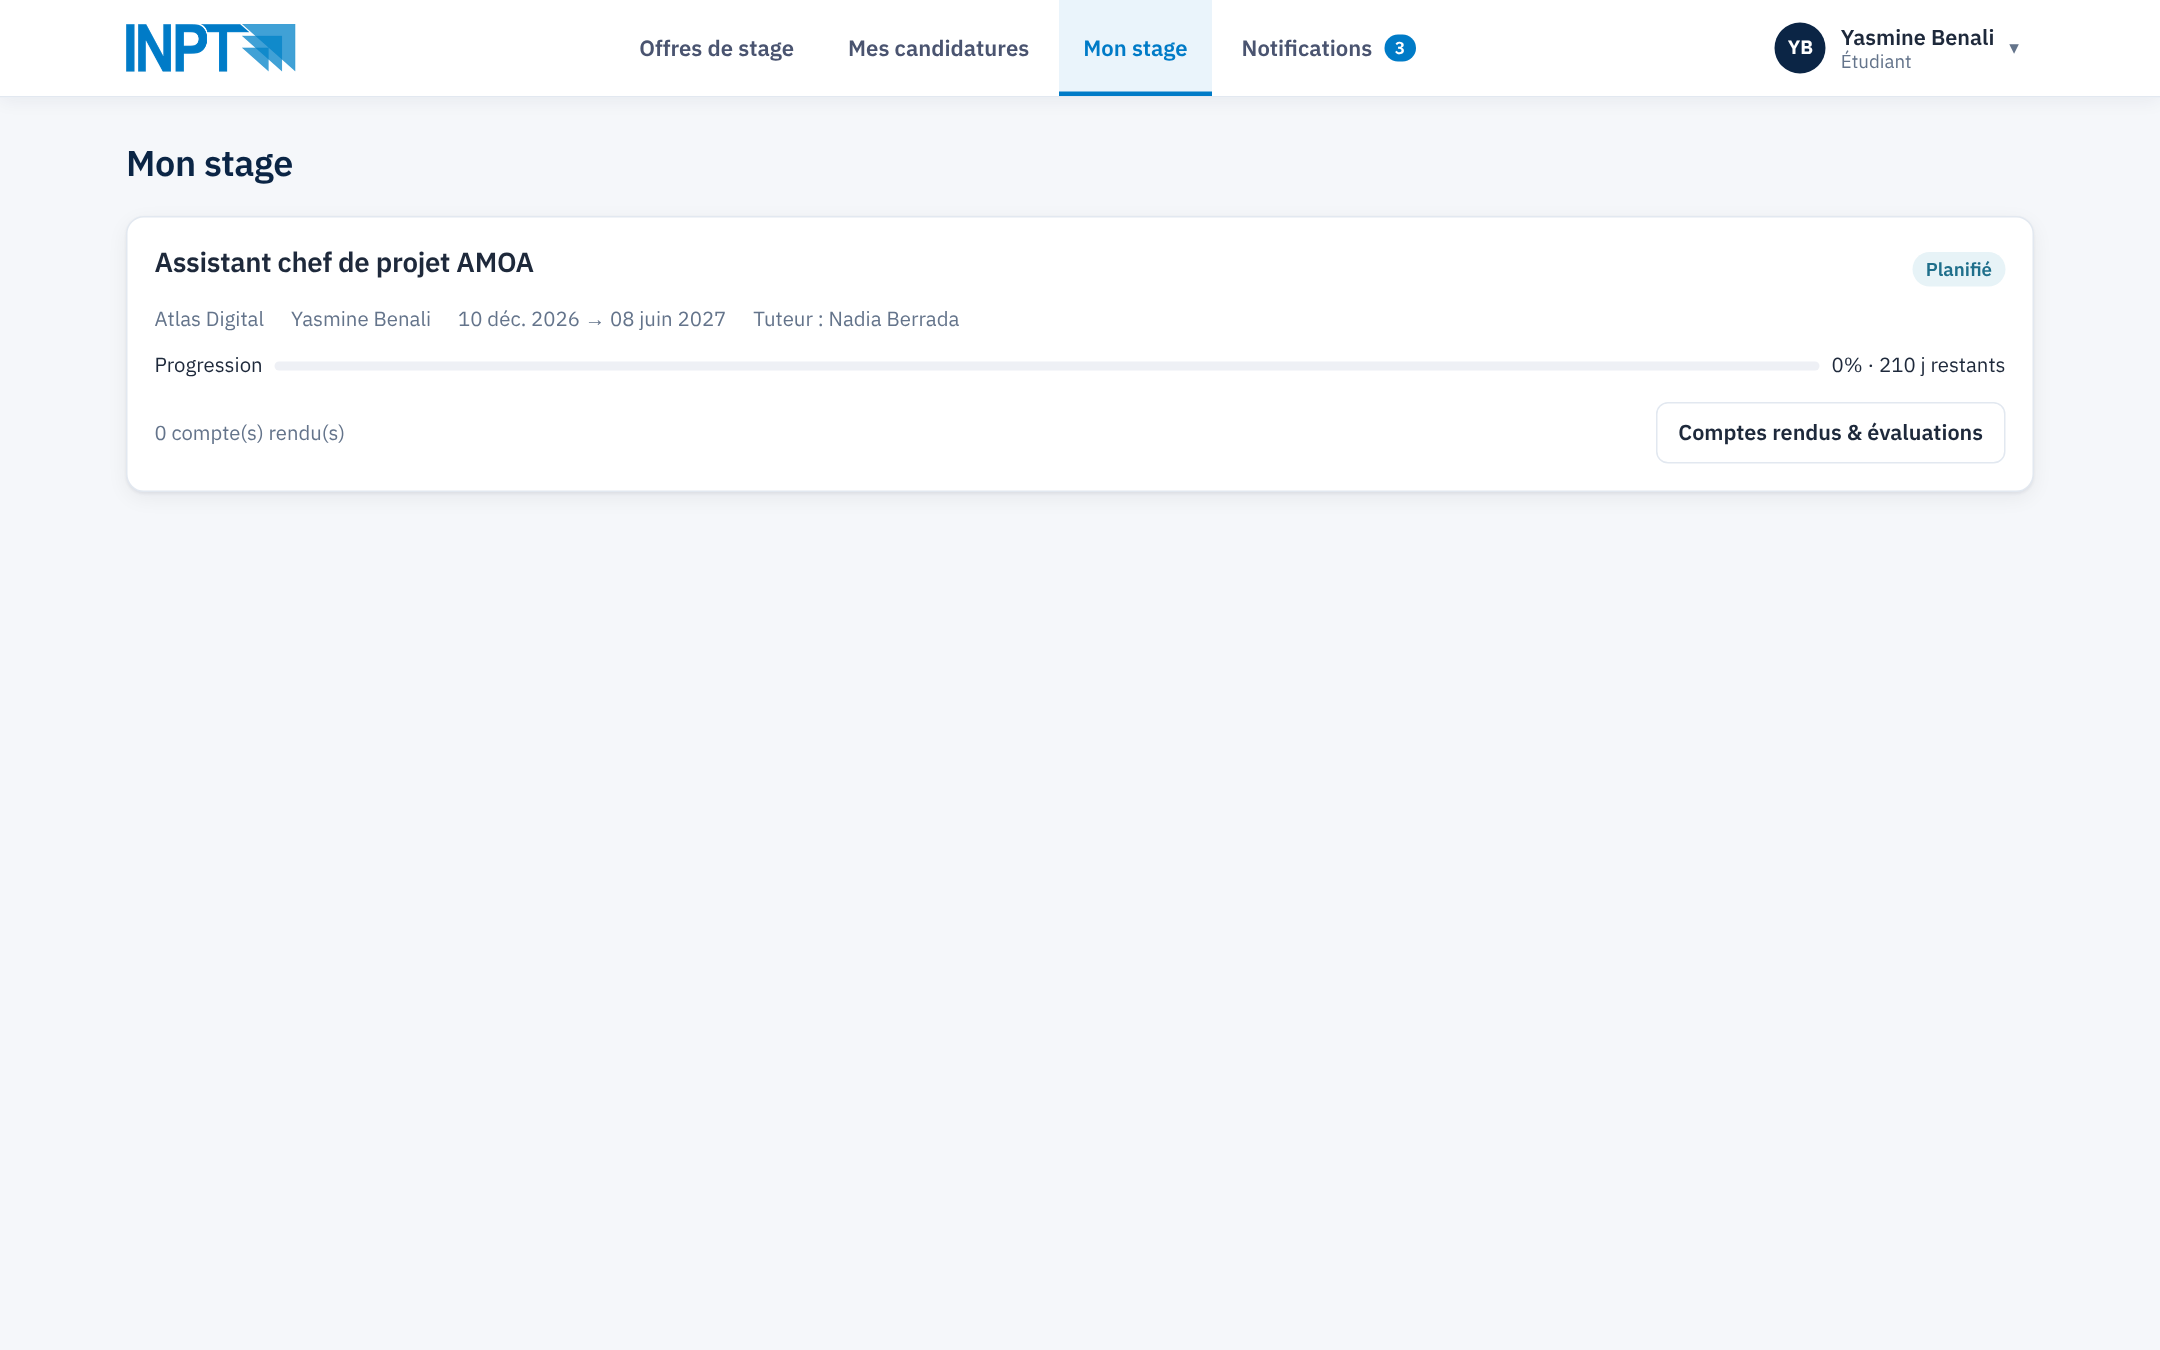
\includegraphics[width=\linewidth]{figures/ui-etudiant-stage.png}\\[-2pt]{\small (b) suivi du stage}
\end{minipage}
\caption{Notifications et suivi du stage}
\end{figure}

\section{E-mails reçus}
\begin{figure}[H]
\centering
\begin{minipage}{0.49\textwidth}\centering
  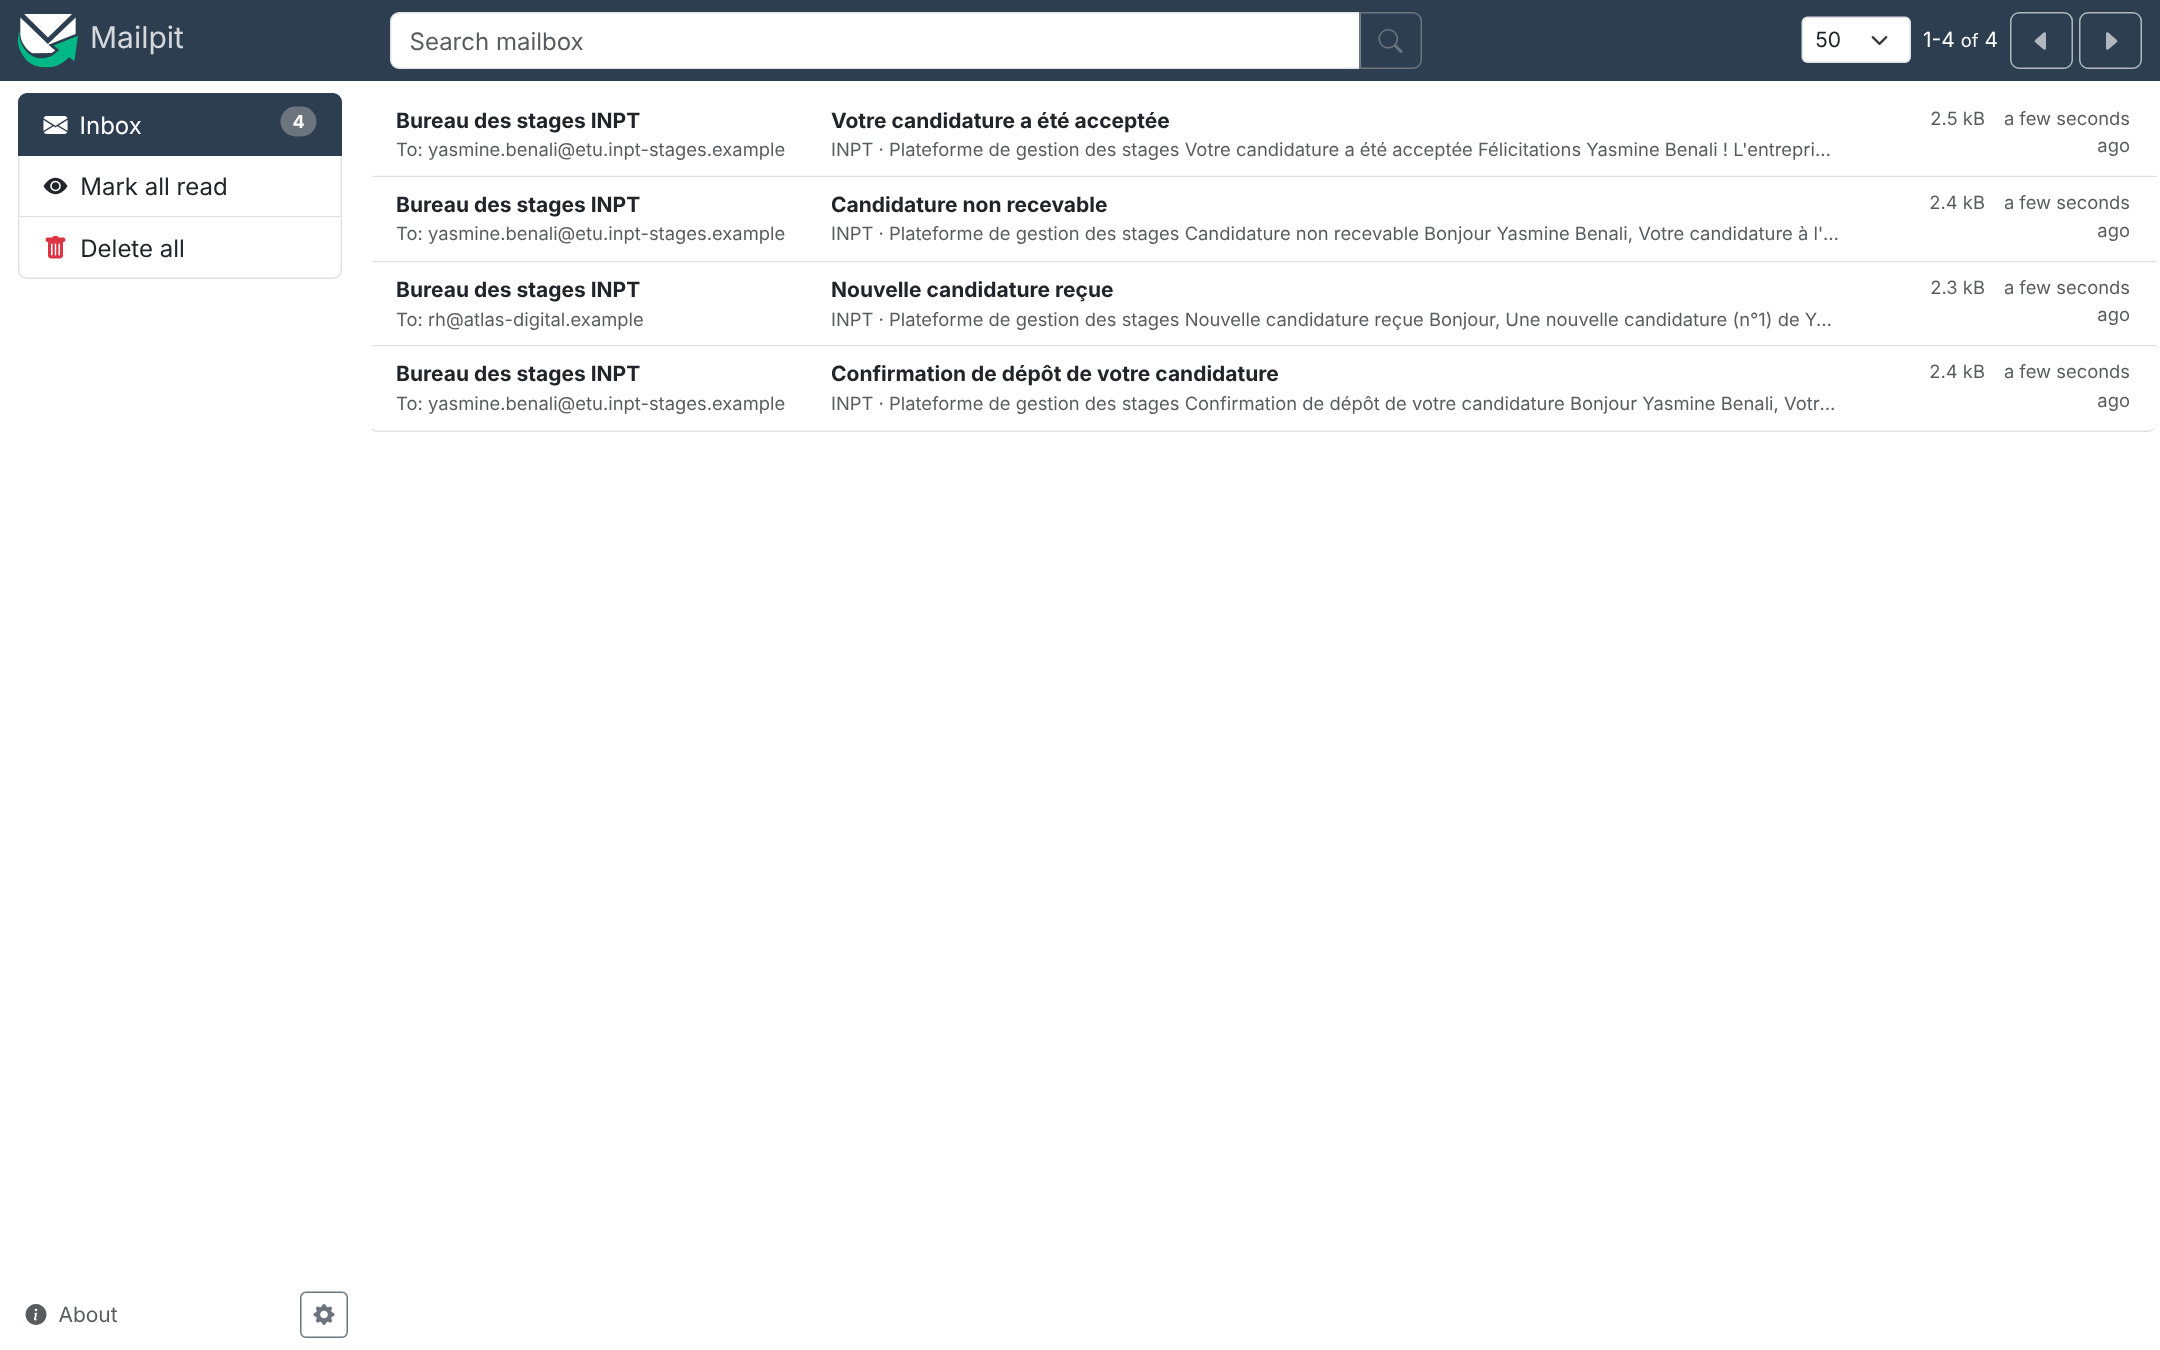
\includegraphics[width=\linewidth]{figures/ui-mailpit-boite.png}\\[-2pt]{\small (a) boîte de réception Mailpit}
\end{minipage}\hfill
\begin{minipage}{0.49\textwidth}\centering
  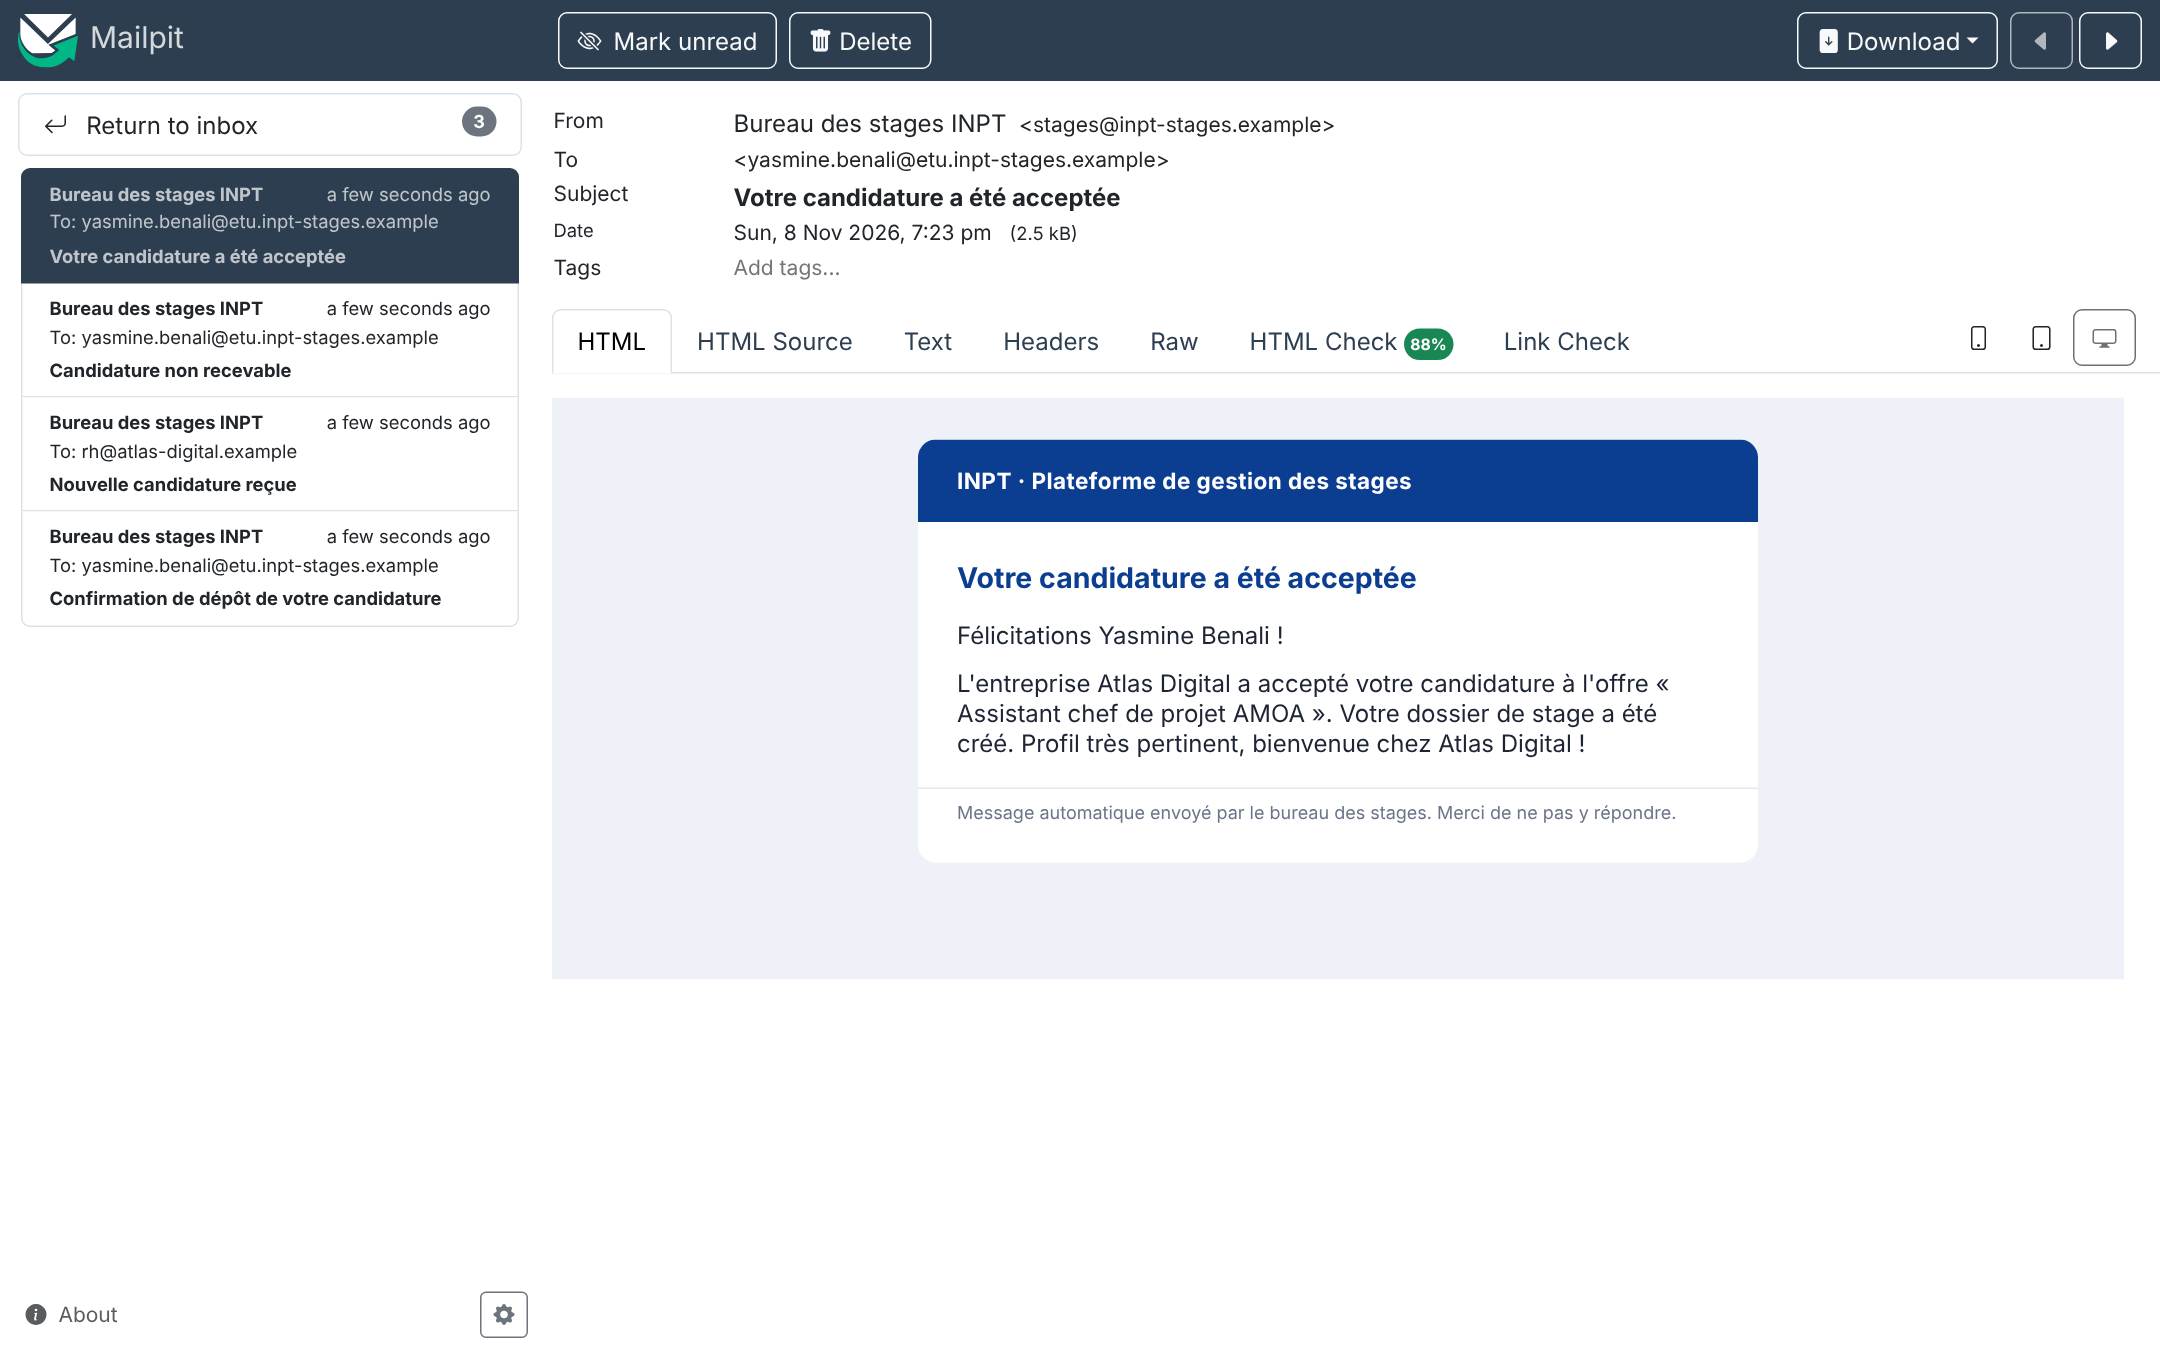
\includegraphics[width=\linewidth]{figures/ui-mailpit-email.png}\\[-2pt]{\small (b) e-mail d'acceptation (HTML)}
\end{minipage}
\caption{Vrais e-mails envoyés en SMTP par le service Notifications et capturés par Mailpit}\label{fig:mailpit}
\end{figure}

\section{Parcours de l'entreprise}
\begin{figure}[H]
\centering
\begin{minipage}{0.49\textwidth}\centering
  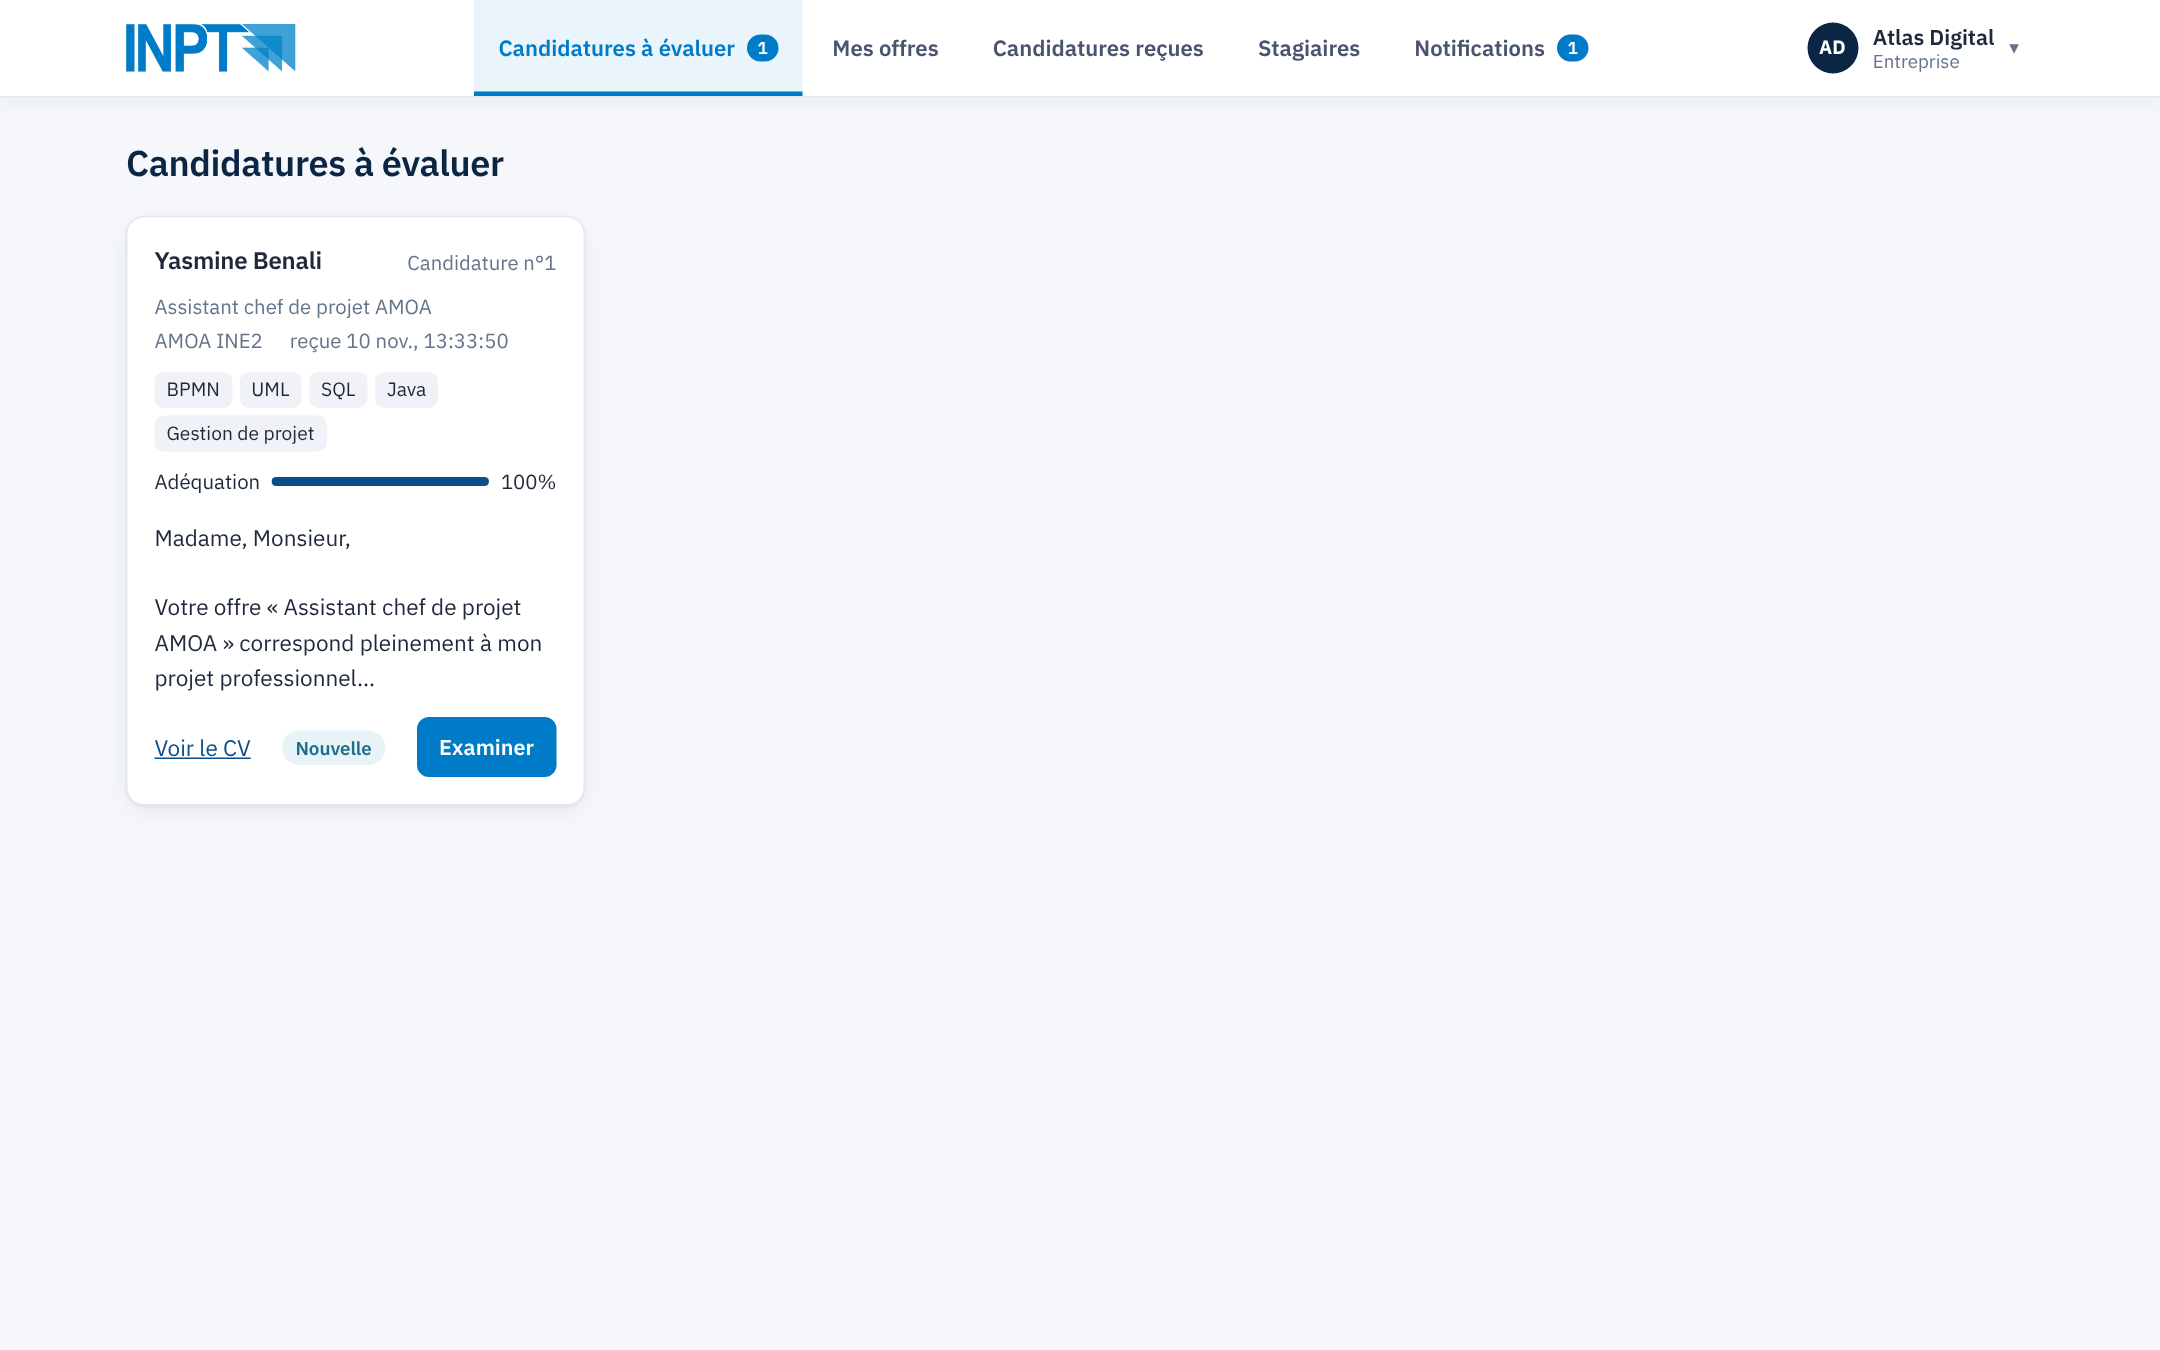
\includegraphics[width=\linewidth]{figures/ui-entreprise-evaluations.png}\\[-2pt]{\small (a) candidatures à évaluer}
\end{minipage}\hfill
\begin{minipage}{0.49\textwidth}\centering
  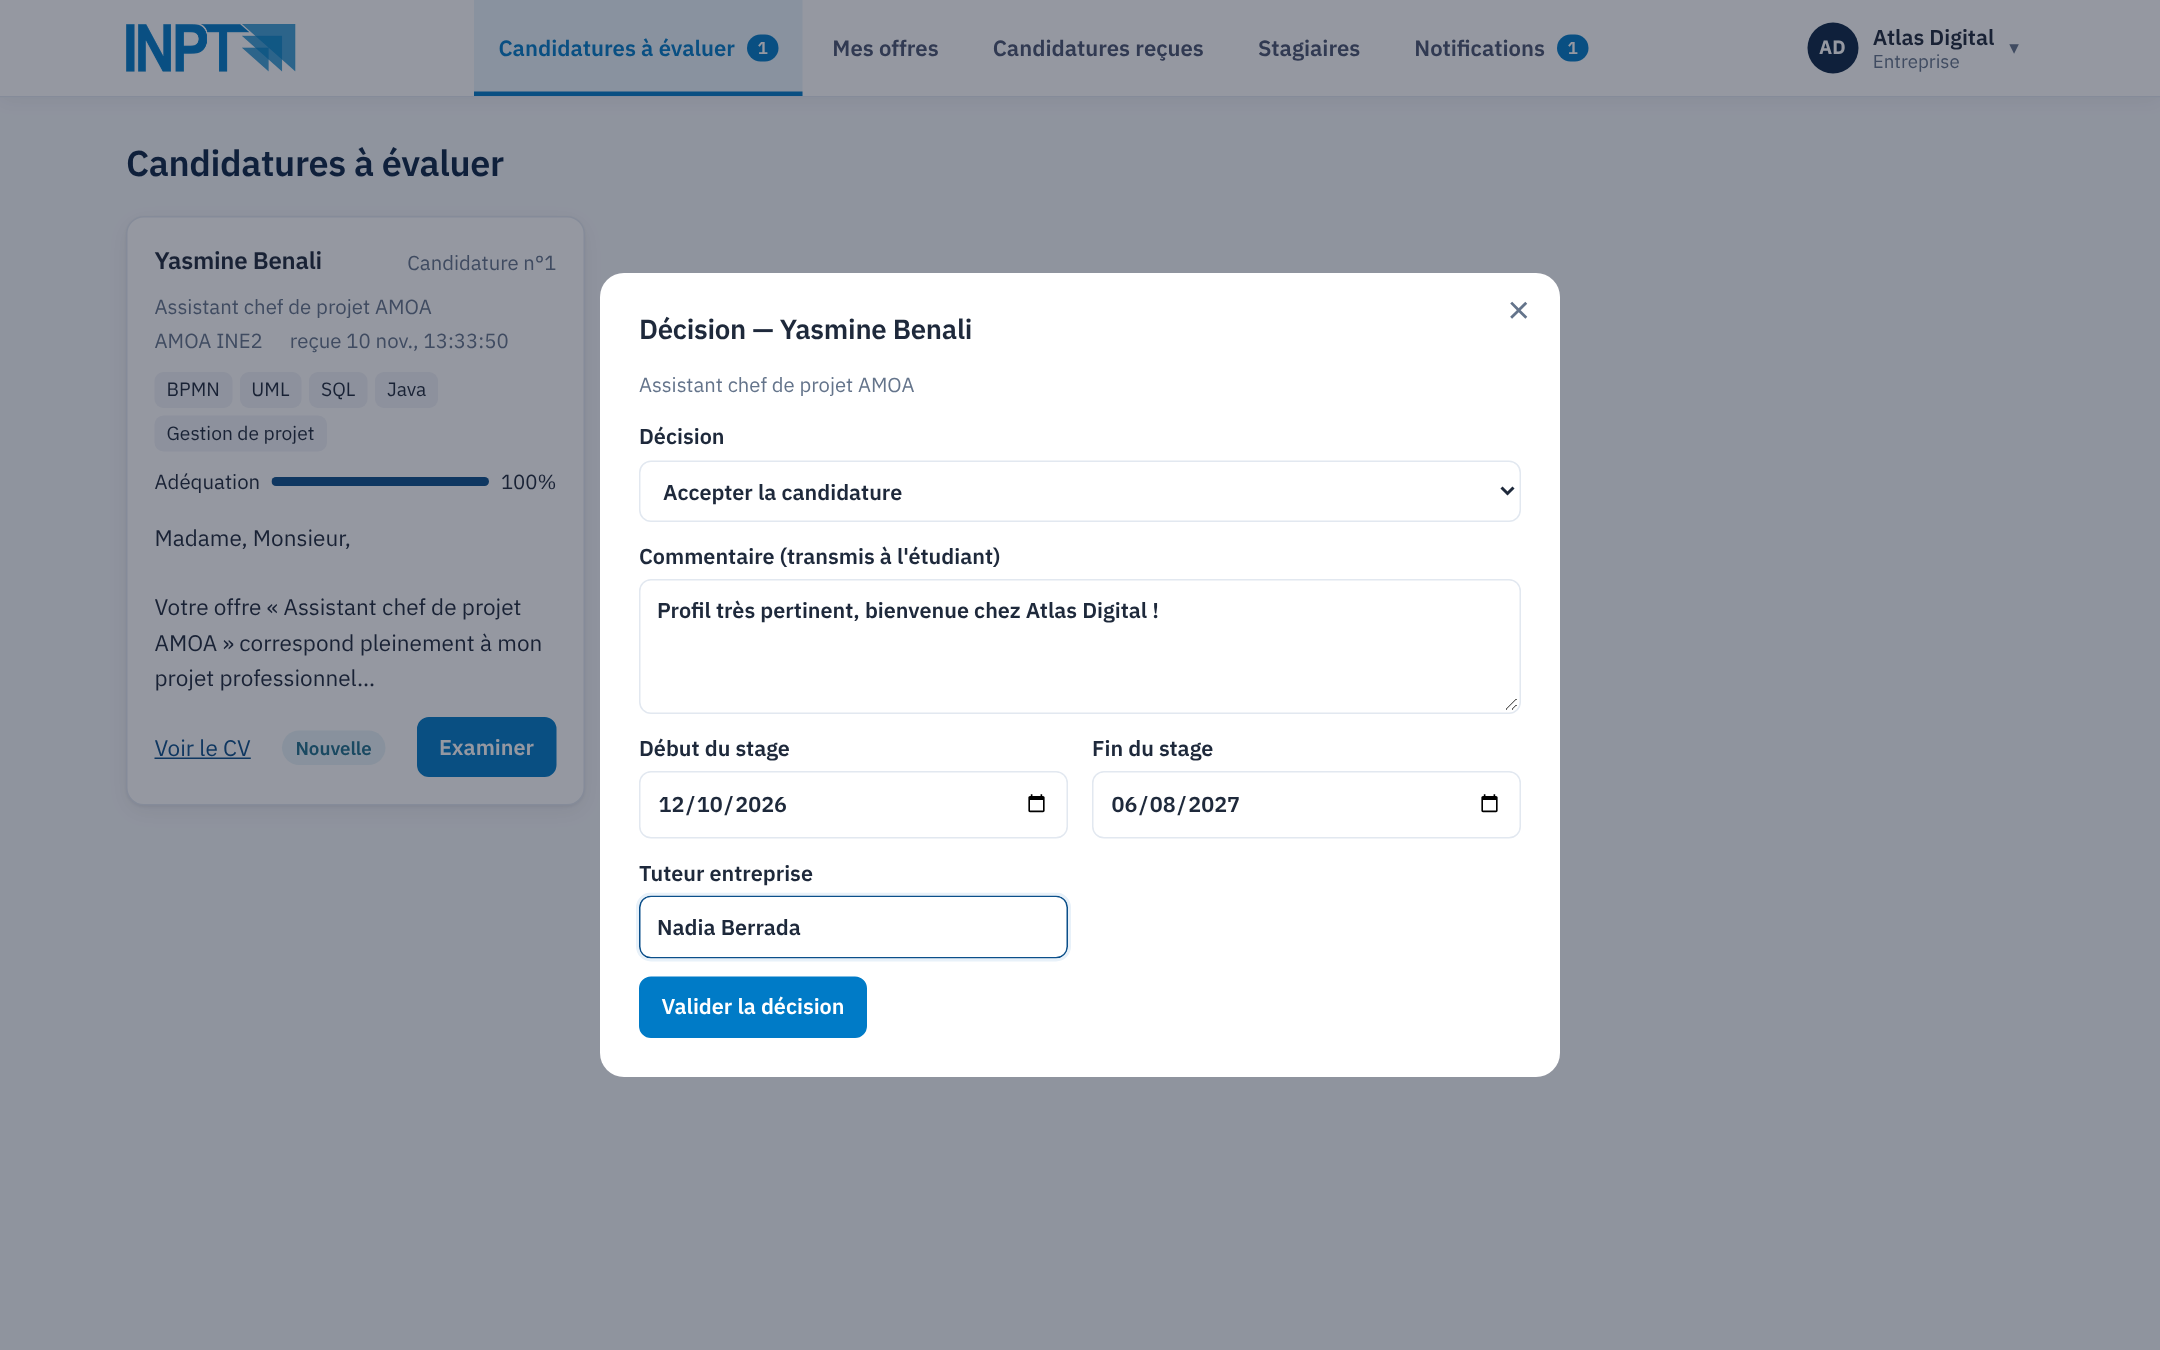
\includegraphics[width=\linewidth]{figures/ui-entreprise-decision.png}\\[-2pt]{\small (b) décision (tâche humaine BPMN)}
\end{minipage}
\caption{Évaluation d'une candidature par l'entreprise : « Examiner » prend la candidature en charge, puis la décision est rendue}
\end{figure}

\section{Parcours du responsable}
\begin{figure}[H]
\centering
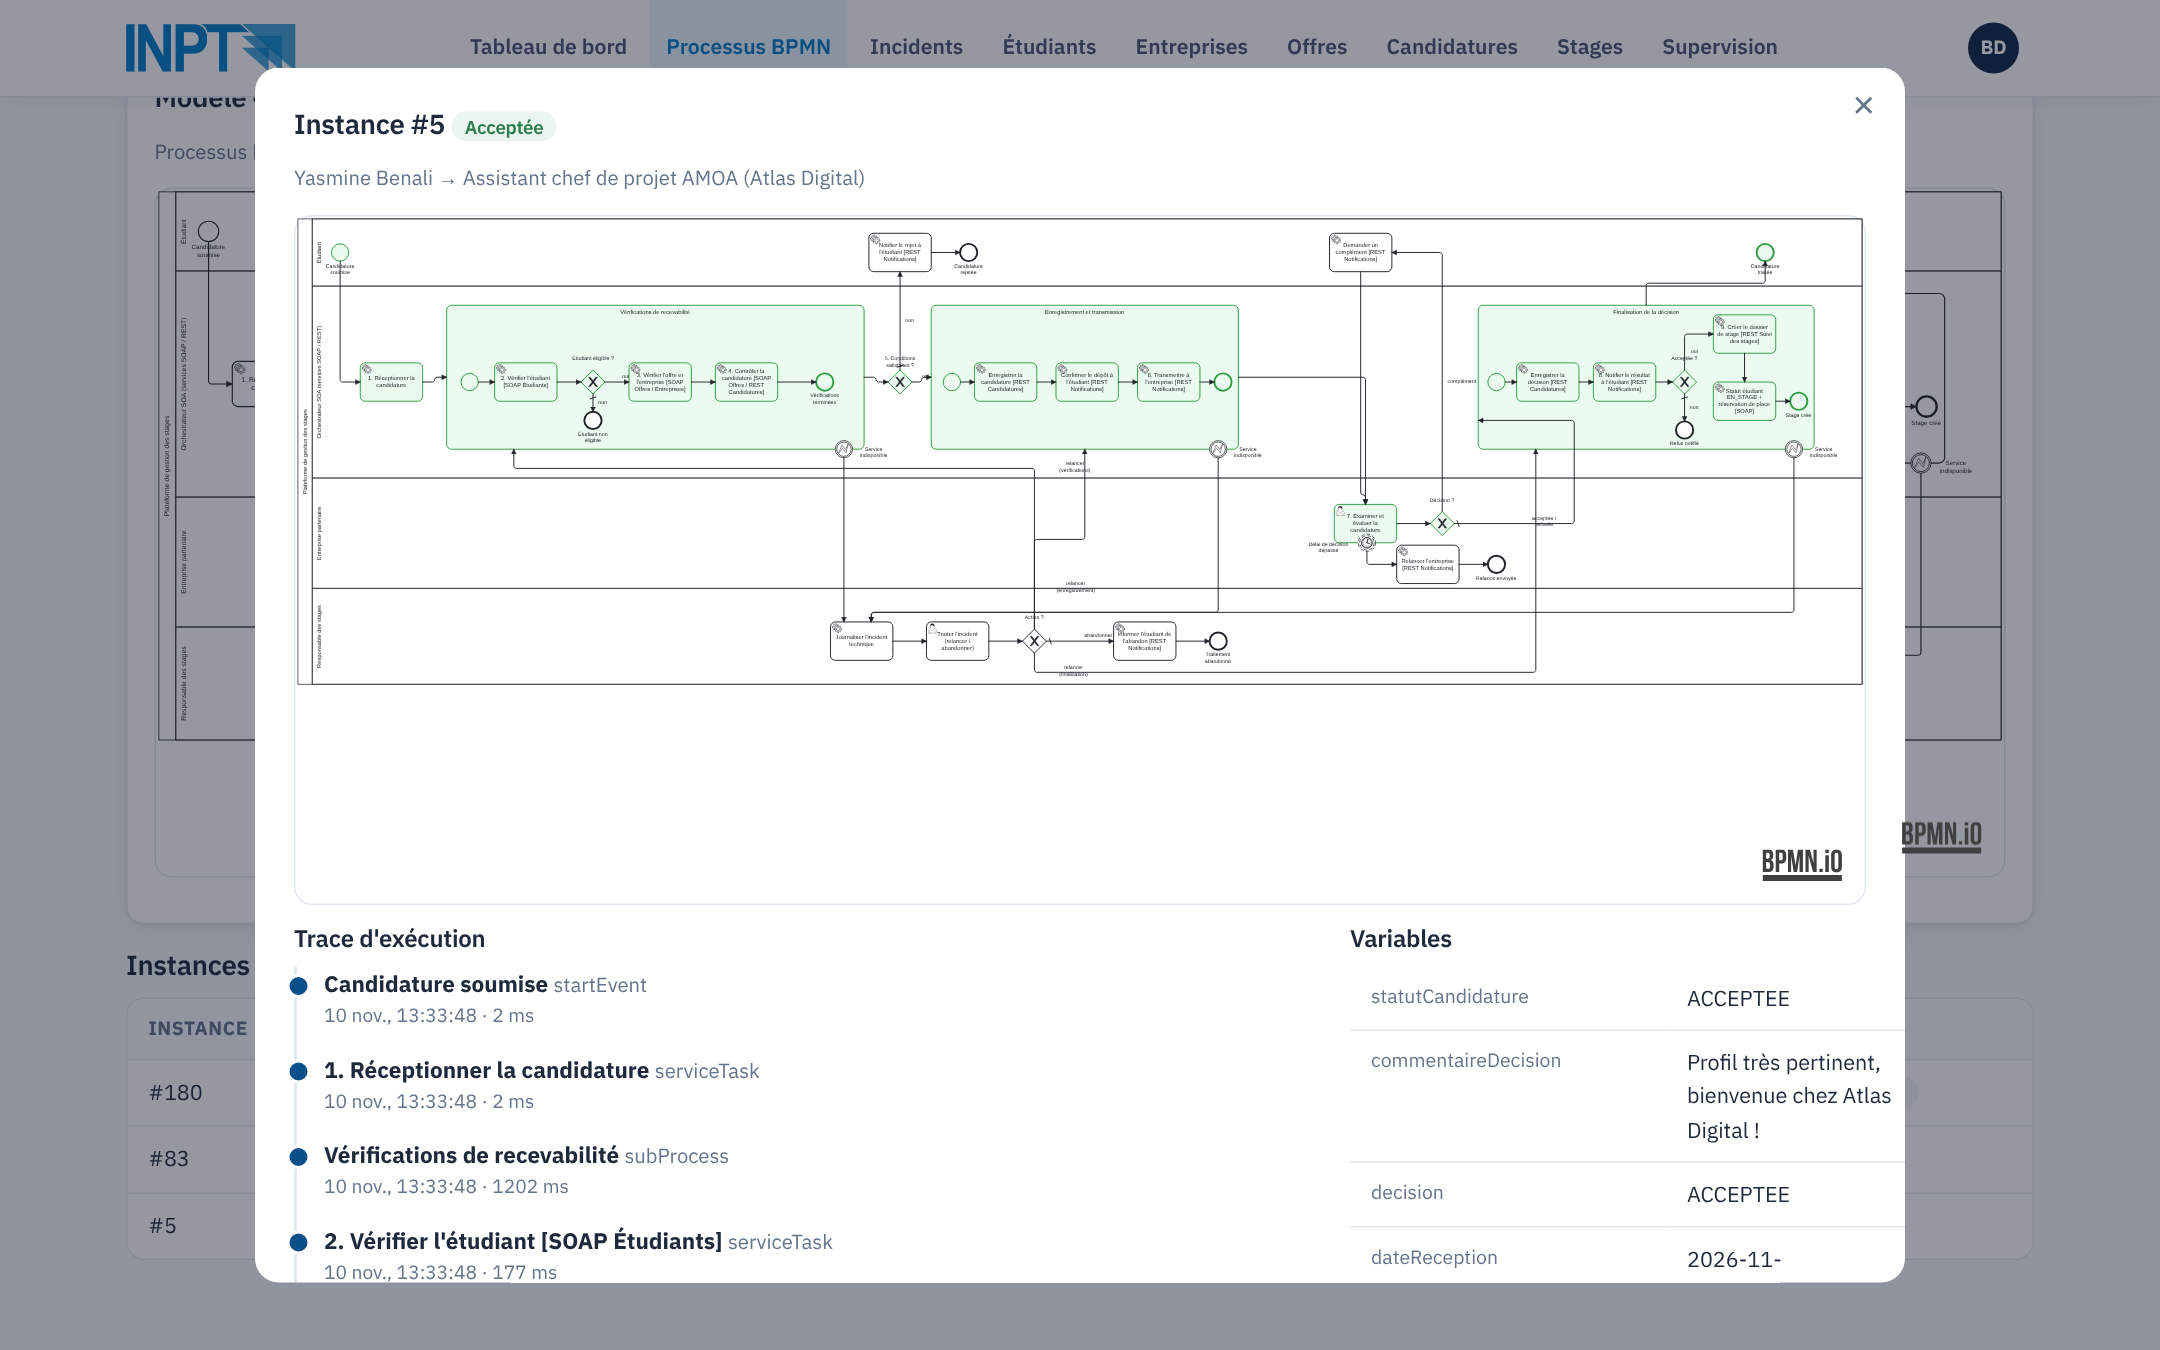
\includegraphics[width=0.92\textwidth]{figures/ui-admin-instance.png}
\caption{Suivi d'une instance : activités traversées en vert sur le diagramme, trace d'exécution et variables}\label{fig:ui-instance}
\end{figure}

\begin{figure}[H]
\centering
\begin{minipage}{0.49\textwidth}\centering
  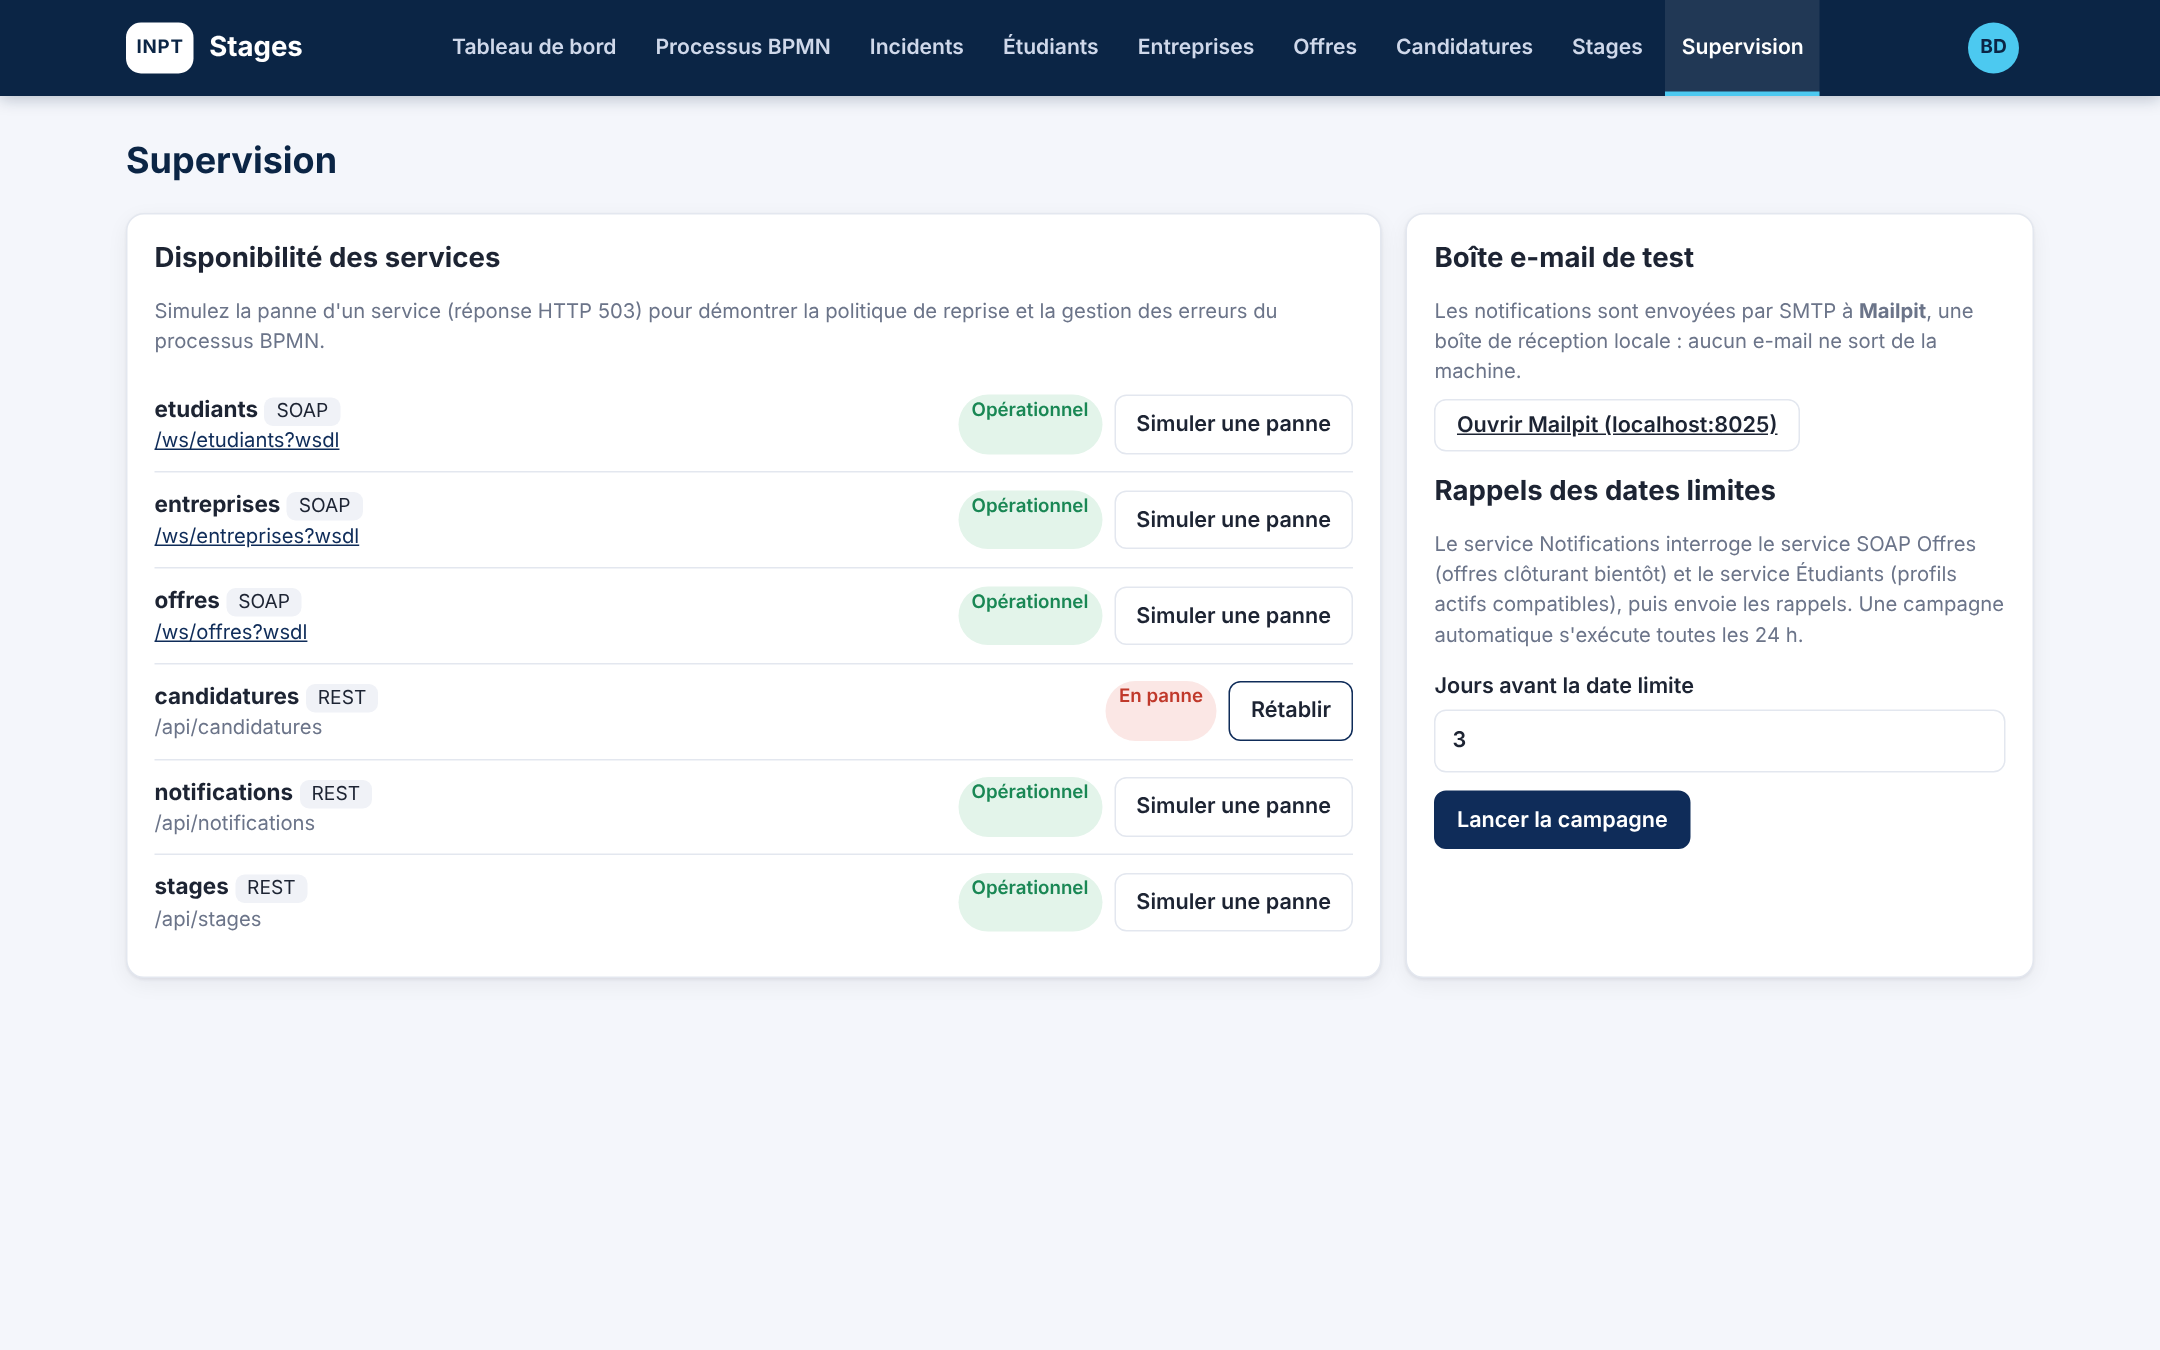
\includegraphics[width=\linewidth]{figures/ui-admin-supervision.png}\\[-2pt]{\small (a) simulation d'une panne}
\end{minipage}\hfill
\begin{minipage}{0.49\textwidth}\centering
  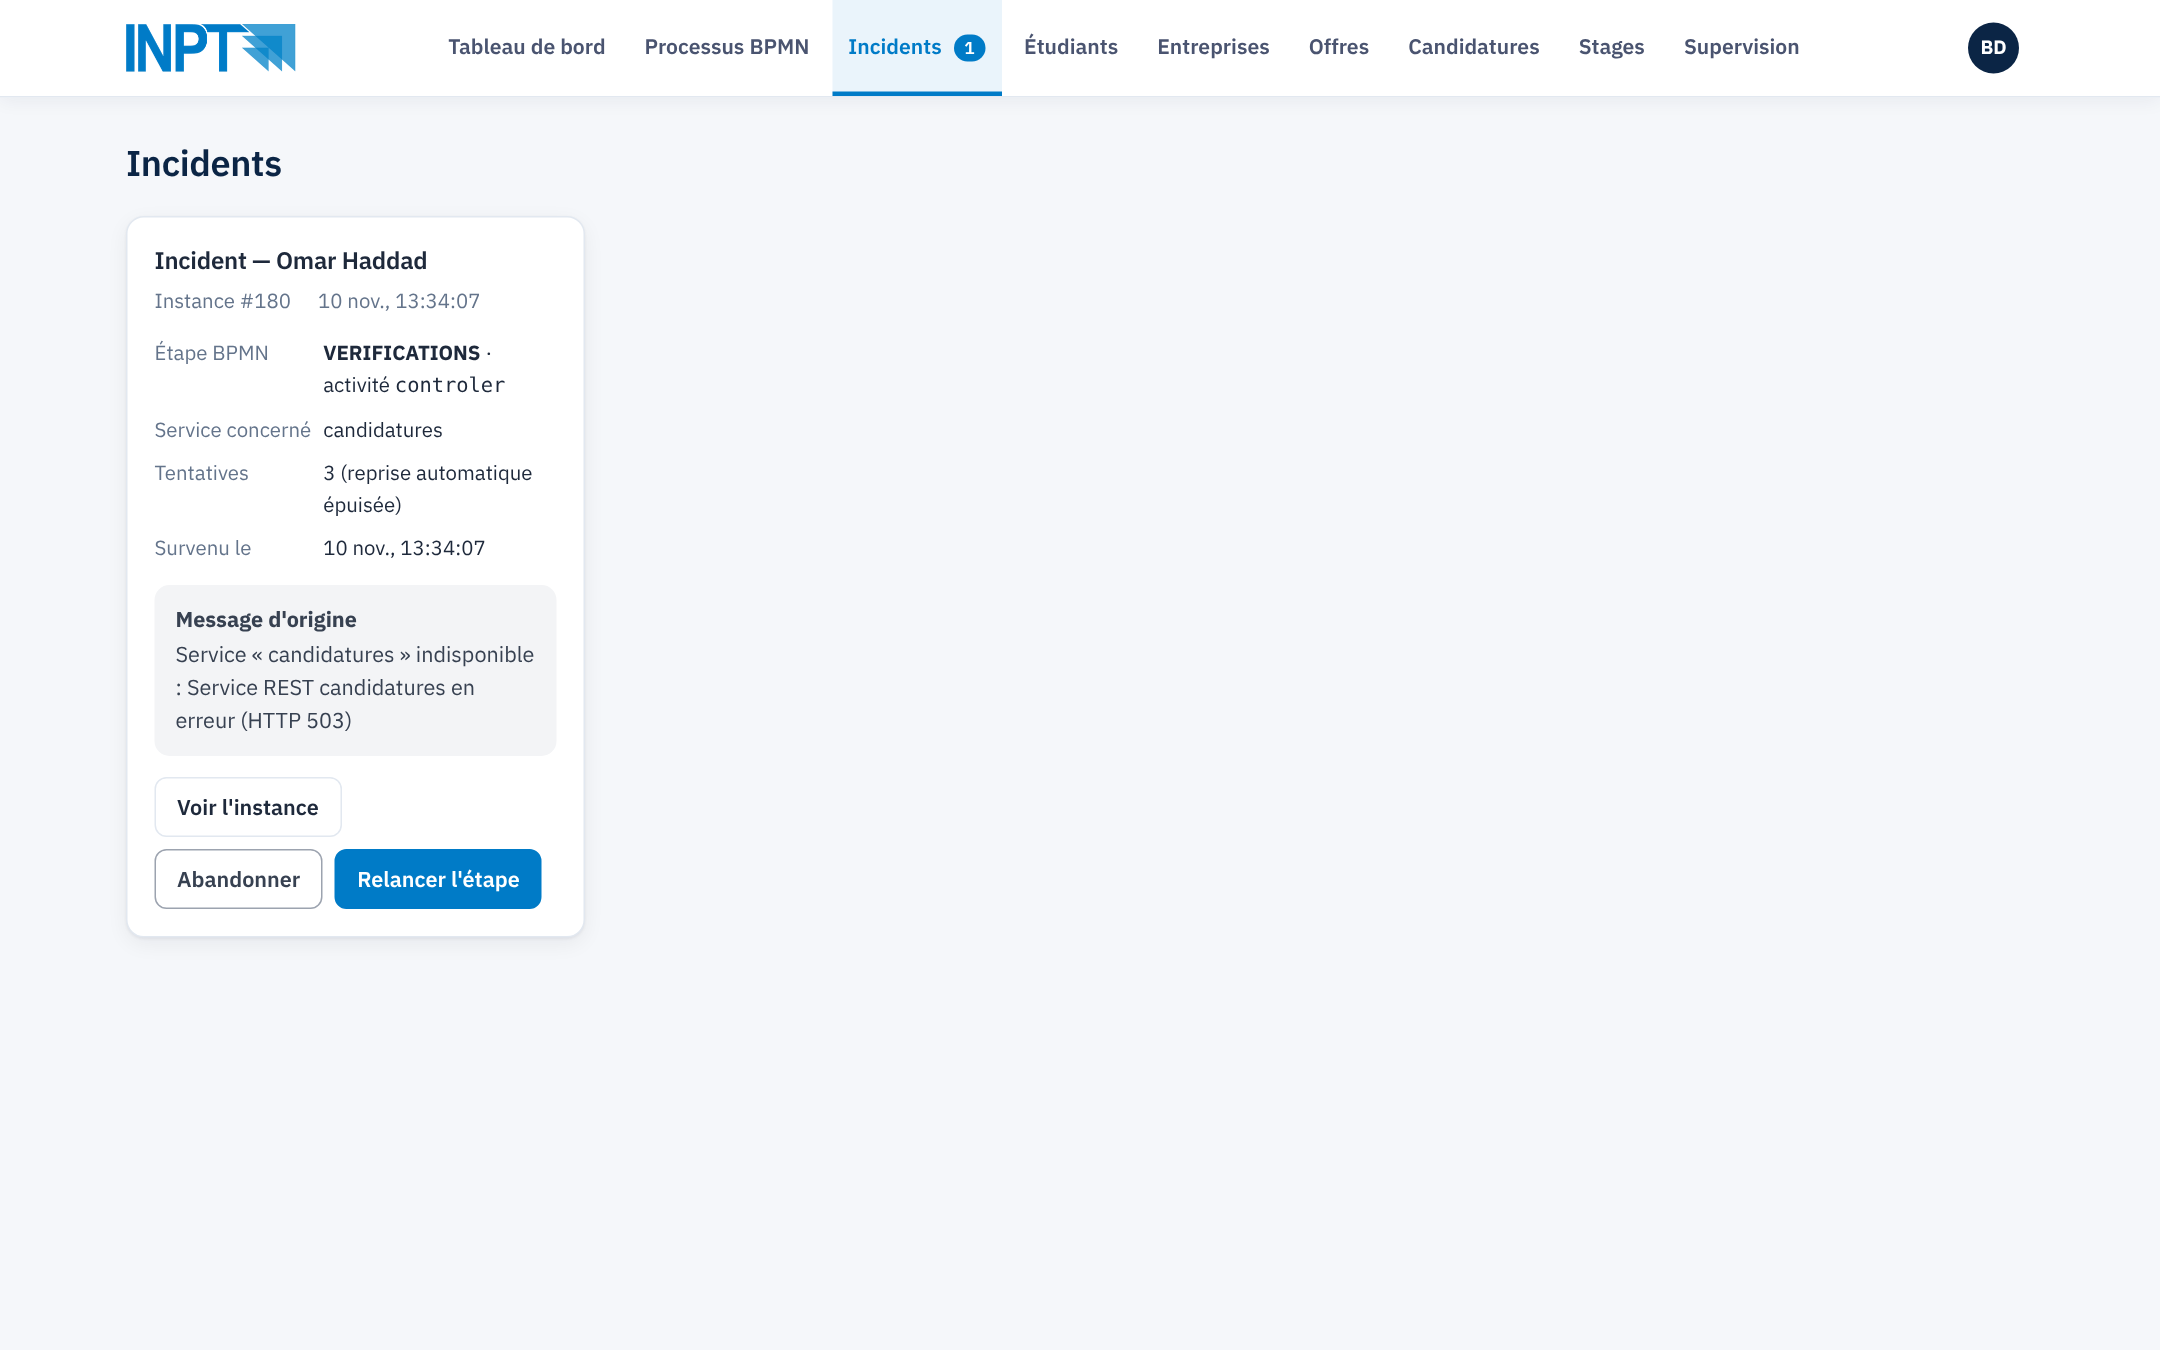
\includegraphics[width=\linewidth]{figures/ui-admin-incidents.png}\\[-2pt]{\small (b) incident à traiter}
\end{minipage}
\caption{Gestion d'une indisponibilité de service depuis l'interface}
\end{figure}

\begin{figure}[H]
\centering
\begin{minipage}{0.49\textwidth}\centering
  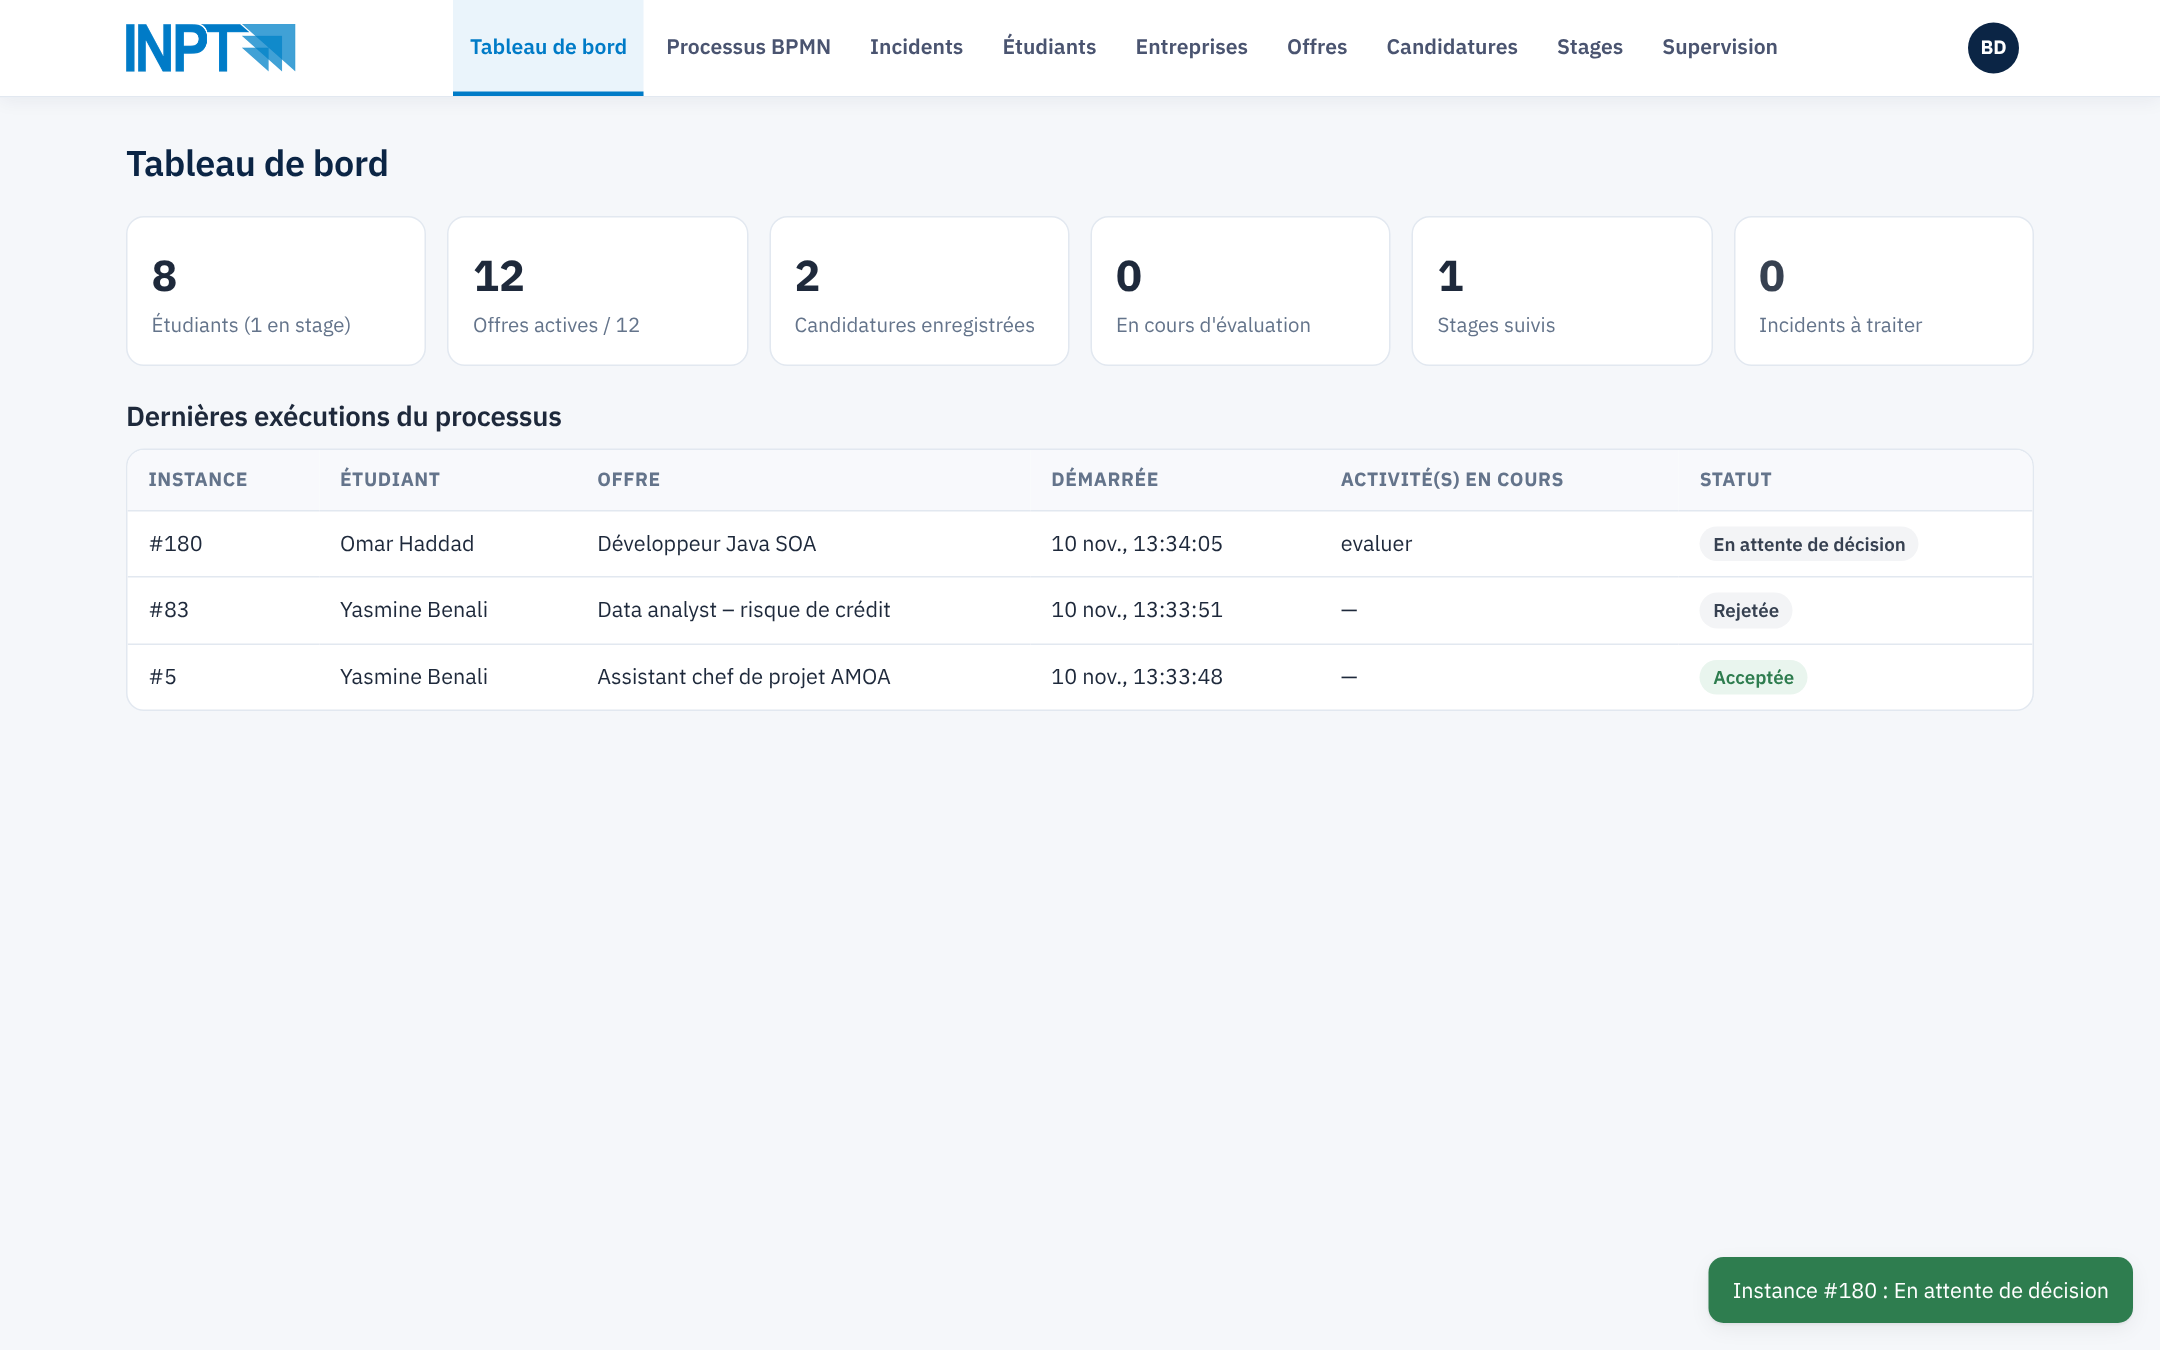
\includegraphics[width=\linewidth]{figures/ui-admin-tableau.png}\\[-2pt]{\small (a) tableau de bord}
\end{minipage}\hfill
\begin{minipage}{0.49\textwidth}\centering
  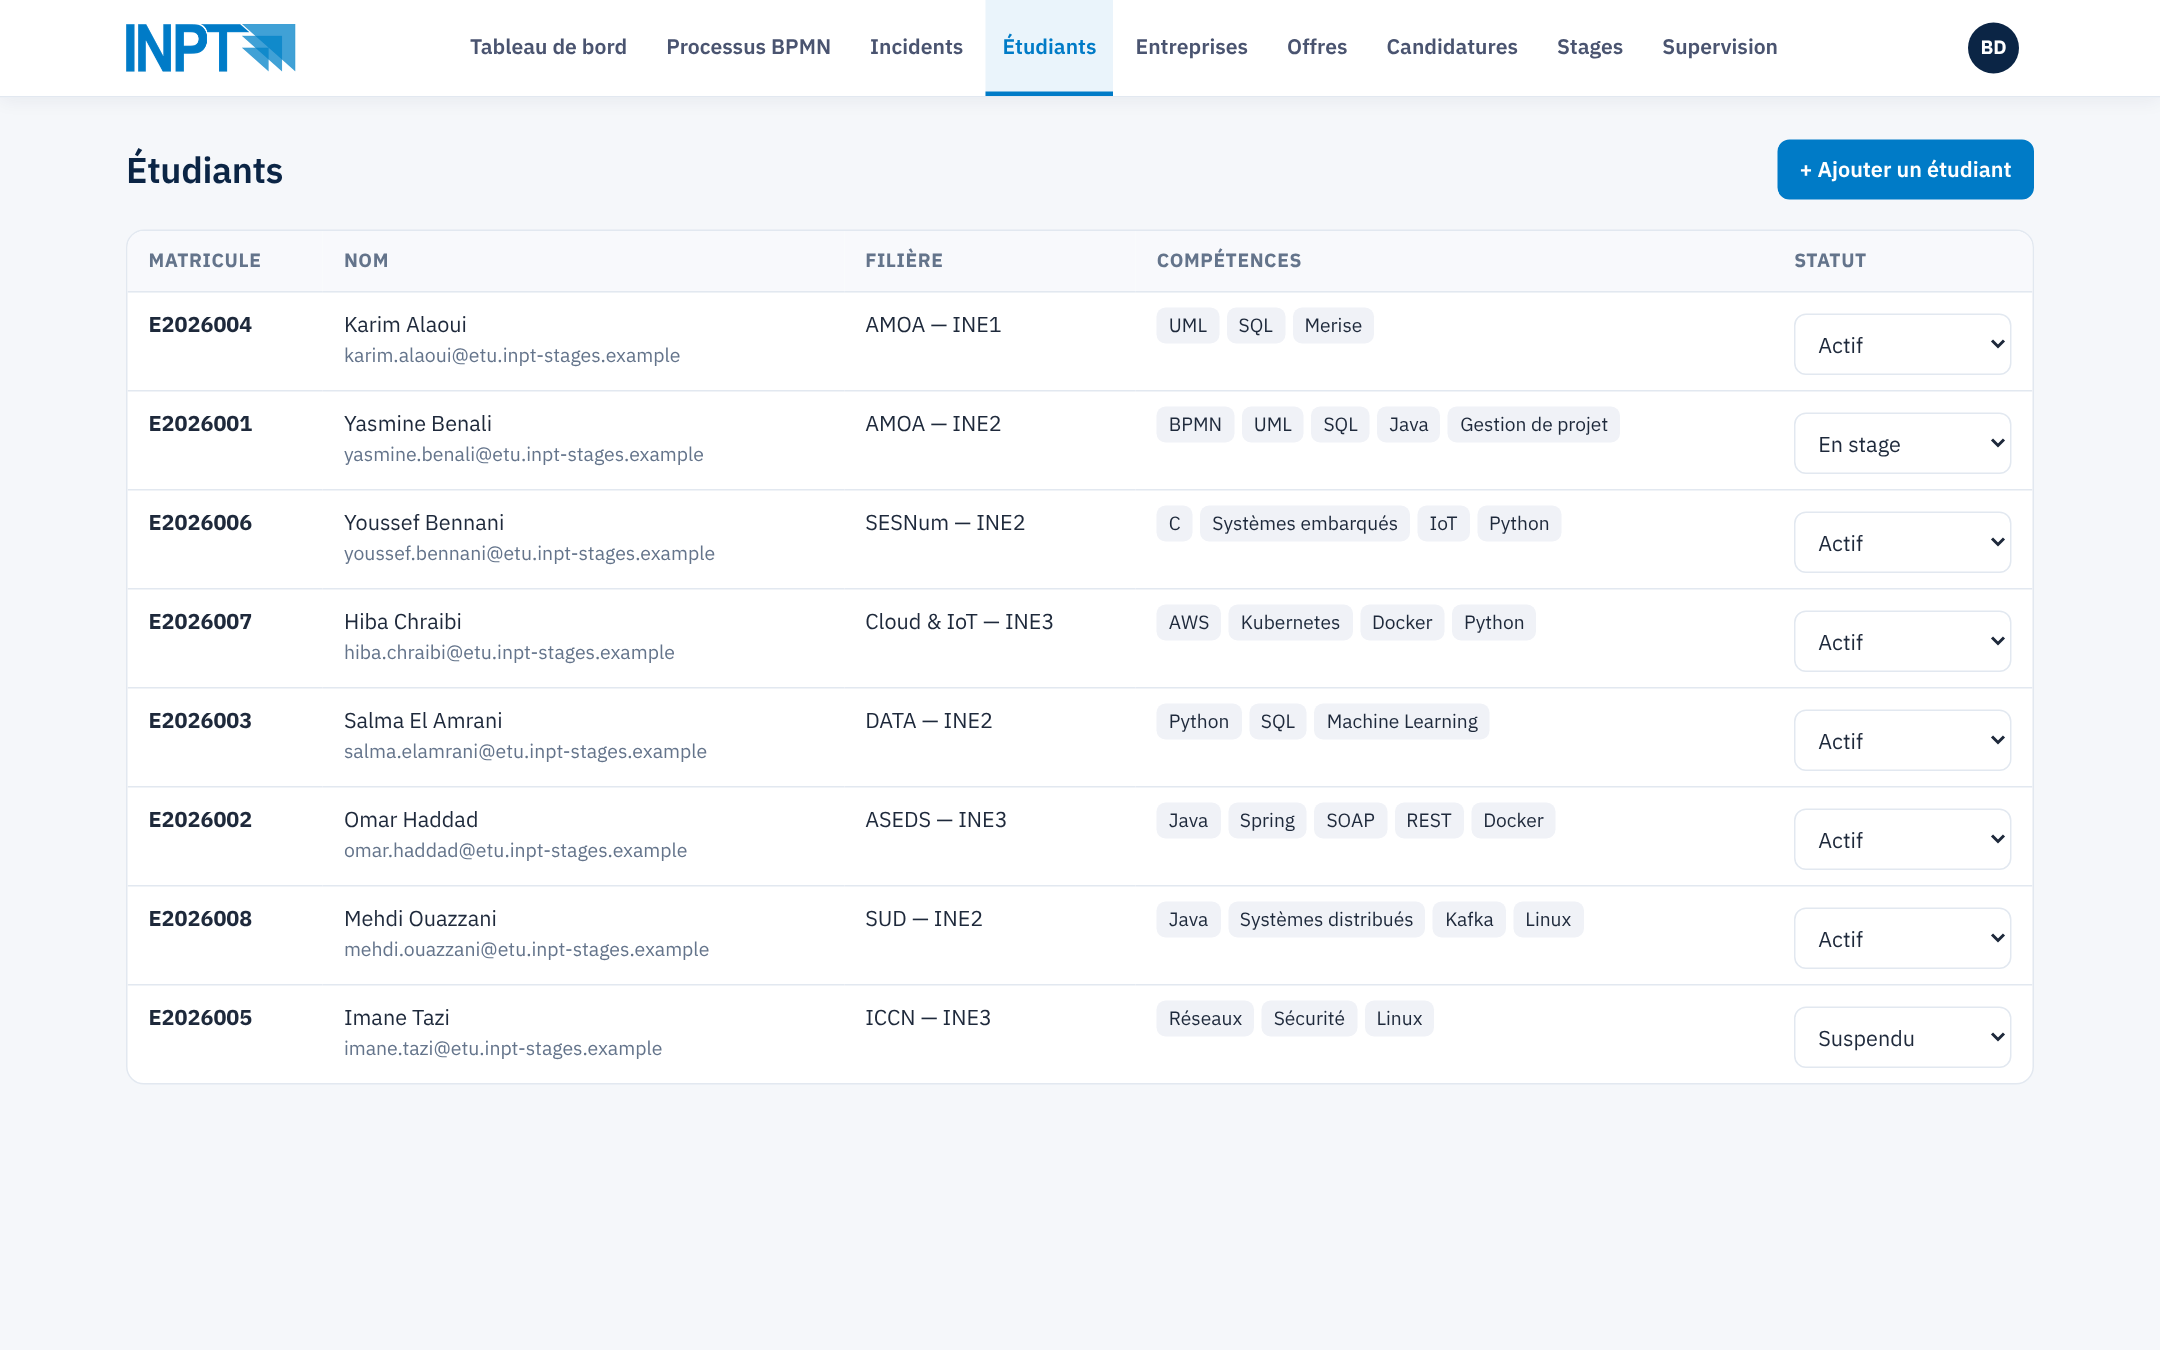
\includegraphics[width=\linewidth]{figures/ui-admin-etudiants.png}\\[-2pt]{\small (b) gestion des étudiants (SOAP)}
\end{minipage}
\caption{Écrans d'administration}
\end{figure}
